%%%%%%%%%%%%%%%%%%%%%%%%%%%%%%%%%%%%%%%%%%%%%%%%%%%%%%%%%%%%%%%%%%%%%%%%
% RAPPORT DE PROJET zz2 2017-2018
% projet : Multiplication de matrices avec MapReduce
% tuteurs : Radu Ciucanu (radu.ciucanu@uca.fr)/Pascal Lafourcade (pascal.lafourcade@uca.fr)/Mathieu Giraud (mathieu.giraud@uca.fr)
% auteurs : Rodrigue Abbe (rodrigue.abbe@etu.uca.fr)/Baptiste Martinez (baptiste.martinez@etu.uca.fr)
%%%%%%%%%%%%%%%%%%%%%%%%%%%%%%%%%%%%%%%%%%%%%%%%%%%%%%%%%%%%%%%%%%%%%%%%

\documentclass[a4paper, 11pt]{article}

% -------------------------------------------------------------------- %
%                                                                      %
% fichier de préambule                                                 %
%                                                                      %
% Importation de nombreux packages, plus francisation                 %
%                                                                      %
% -------------------------------------------------------------------- %

% ----------------------------------------------------------------------
% gestion du français, et des accents
\usepackage{cmap}
\usepackage[T1]{fontenc}
\usepackage[english,frenchb]{babel}
\usepackage[utf8]{inputenc}
\usepackage{helvet}
\usepackage{courier}
\usepackage{rotating}
%\renewcommand{\familydefault}{\sfdefault}
%\pdfcompresslevel=3
%\usepackage{fourier}

\usepackage{datetime} % pour avoir l'heure de compilation avec \currenttime
%\newcommand{mydate}{20}{mars}{2018}

\usepackage{color}
\usepackage[table]{xcolor}

\usepackage{sectsty}
\usepackage{pdfpages}
\allsectionsfont{\bfseries\sffamily\color{black!90}\hspace{-1em}}
\partfont{\sffamily}
\usepackage[font={small,it}]{caption}
\makeatletter
\def\@seccntformat#1{\llap{\csname the#1\endcsname\quad}}
\makeatletter\pdfcompresslevel=9
\def\@seccntformat#1{\llap{\csname the#1\endcsname\quad}}
\makeatother

% ----------------------------------------------------------------------
% bibliography
\usepackage[backend=biber, bibencoding=utf8 , sorting=none,hyperref=true,url=false,backref=true,backrefstyle=three]{biblatex}
\bibliography{input/biblio}

% ----------------------------------------------------------------------
% packages pour les figures
\usepackage{graphicx}
\usepackage{subfig}
\usepackage{tikz}

% change la numéroration des figures
%%%% debut macro %%%%
\makeatletter
\renewcommand{\thefigure}{\ifnum \c@section>\z@ \thesection.\fi
 \@arabic\c@figure}
\@addtoreset{figure}{section}
\makeatother
%%%% fin macro %%%%

% change la numéroration des tableaux
%%%% debut macro %%%%
\makeatletter
\renewcommand{\thetable}{\ifnum \c@section>\z@ \thesection.\fi
 \@arabic\c@table}
\@addtoreset{table}{section}
\makeatother
%%%% fin macro %%%%

% ----------------------------------------------------------------------
% diagramme de Gantt
%\usepackage{model/pgfgantt}

% ----------------------------------------------------------------------
% pour mettre une page en mode paysage
\usepackage{lscape}

% ----------------------------------------------------------------------
% Miscelianous
\usepackage[pdfborder={0 0 0 [3 3]},pdftex,unicode=true]{hyperref}
\usepackage{bookmark}

%\usepackage{tablefootnote}

% ----------------------------------------------------------------------
%packages pour les maths
\usepackage{amsmath}
\usepackage{amssymb}
\usepackage{mathabx} %   \ldbrack et \rdbrack
%\usepackage{amsfonts}
\usepackage{mathrsfs}
\usepackage{wasysym}
\usepackage{textcomp}
%\usepackage{bbm}
\DeclareMathAlphabet{\mathpzc}{OT1}{pzc}{m}{it} % \mathpzc{ABCdef}
\usepackage{eufrak}                             % \mathfrak{ABCdef}

% change la numéroration des équations
\numberwithin{equation}{section}

% ----------------------------------------------------------------------
% pour les unités
%\usepackage[load=physical]{siunitx}
\newcommand{\eV}{\mathrm{eV}}
\newcommand{\s}{\mathrm{s}}
\newcommand{\m}{\mathrm{m}}
\newcommand{\g}{\mathrm{g}}
\newcommand{\V}{\mathrm{V}}
\newcommand{\sample}{\mathrm{s}}
\newcommand{\Hz}{\mathrm{Hz}}
\newcommand{\pc}{\mathrm{pc}}

\newcommand{\nano}{\mathrm{n}}
\newcommand{\micro}{\mathrm{\mu}}
\newcommand{\milli}{\mathrm{m}}
\newcommand{\centi}{\mathrm{c}}
\newcommand{\kilo}{\mathrm{k}}
\newcommand{\mega}{\mathrm{M}}
\newcommand{\giga}{\mathrm{G}}
\newcommand{\tera}{\mathrm{T}}
\newcommand{\exa}{\mathrm{E}}
\newcommand{\zetta}{\mathrm{Z}}


% ----------------------------------------------------------------------
% packages pour les algorithmes
\usepackage[section]{algorithm}
\usepackage[noend]{algpseudocode}

\renewcommand{\algorithmiccomment}[1]{{\hfill$\vartriangleright$\scriptsize\sffamily~ #1}}

% francisation des algorithmes
\floatname{algorithm}{\sffamily Algorithme}

\renewcommand{\algorithmicprocedure} {{\footnotesize \textbf{\textsf{Proc\'edure}} }}
\renewcommand{\algorithmicwhile}     {{\footnotesize \textbf{\textsf{Tant que}}    }}
\renewcommand{\algorithmicdo}        {{\footnotesize \textbf{\textsf{Faire}}       }}
\renewcommand{\algorithmicend}       {{\footnotesize \textbf{\textsf{Fin}}         }}
\renewcommand{\algorithmicif}        {{\footnotesize \textbf{\textsf{Si}}          }}
\renewcommand{\algorithmicelse}      {{\footnotesize \textbf{\textsf{Sinon}}       }}
\renewcommand{\algorithmicthen}      {{\footnotesize \textbf{\textsf{Alors}}       }}
\renewcommand{\algorithmicfor}       {{\footnotesize \textbf{\textsf{Pour}}        }}
\renewcommand{\algorithmicforall}    {{\footnotesize \textbf{\textsf{Pour tout}}   }}
\renewcommand{\algorithmicdo}        {{\footnotesize \textbf{\textsf{Faire}}       }}
\renewcommand{\algorithmicrepeat}    {{\footnotesize \textbf{\textsf{Répéter}}     }}
\renewcommand{\algorithmicuntil}     {{\footnotesize \textbf{\textsf{Jusqu'à}}     }}
\renewcommand{\algorithmicfunction}  {{\footnotesize \textbf{\textsf{Fonction}}    }}
\renewcommand{\algorithmicreturn}    {{\footnotesize \textbf{\textsf{Retourner}}   }}
\let\mylistof\listof
\renewcommand\listof[2]{\mylistof{algorithm}{Liste des algorithmes}}
\makeatletter
\providecommand*{\toclevel@algorithm}{0}
\makeatother
% Lister les algorithmes :
%\listofalgorithms % même principe que toc
\addto\captionsfrench{%
  \renewcommand{\listfigurename}{Liste des figures}%
}
\addto\captionsfrench{\def\figurename{Figure}}
\addto\captionsfrench{\def\tablename{Tableau}}

% ----------------------------------------------------------------------
% tableaux
\definecolor{tablegray}{gray}{0.8}%table

% ----------------------------------------------------------------------
% importantion de code
\definecolor{mygray}{rgb}{0.5,0.5,0.5} % définition du gris (n° ligne)
\usepackage{listings}
\usepackage{listingsutf8}

% pour la numerotation des codes
\usepackage{chngcntr}
\AtBeginDocument{\counterwithin{lstlisting}{section}}

\renewcommand{\lstlistlistingname}{Liste des extraits de code}
%%options for listings
\DeclareCaptionFont{white}{\color{white}}
\DeclareCaptionFormat{listing}{\colorbox{black!80}{\parbox{\textwidth}{#1#2#3}}}
\captionsetup[lstlisting]{format=listing,labelfont={white,tt},textfont=white}
\definecolor{Rred}{rgb}{0.6,0,0} % for strings
\definecolor{Rgreen}{rgb}{0.25,0.5,0.35} % comments
\definecolor{Rpurple}{rgb}{0.5,0,0.35} % keywords
\definecolor{Rdocblue}{rgb}{0.25,0.35,0.75} % Rdoc
\lstset{
    float,
    columns=fullflexible,
    numbers=left,
    tabsize=2,
    breaklines=true,
    basicstyle=\small\ttfamily,
    basewidth=0.51em,
    showspaces=false,
    showstringspaces=false,
    stringstyle=\color{Rred},
    commentstyle=\color{Rgreen},
    keywordstyle=\color{Rdocblue}
}
% gestion des accents dans le code
\renewcommand{\lstlistingname}{Code}
\lstset{literate=
    {á}{{\'a}}1 {é}{{\'e}}1 {í}{{\'i}}1 {ó}{{\'o}}1 {ú}{{\'u}}1
    {Á}{{\'A}}1 {É}{{\'E}}1 {Í}{{\'I}}1 {Ó}{{\'O}}1 {Ú}{{\'U}}1
    {à}{{\`a}}1 {è}{{\`e}}1 {ì}{{\`i}}1 {ò}{{\`o}}1 {ù}{{\`u}}1
    {À}{{\`A}}1 {È}{{\'E}}1 {Ì}{{\`I}}1 {Ò}{{\`O}}1 {Ù}{{\`U}}1
    {ä}{{\"a}}1 {ë}{{\"e}}1 {ï}{{\"i}}1 {ö}{{\"o}}1 {ü}{{\"u}}1
    {Ä}{{\"A}}1 {Ë}{{\"E}}1 {Ï}{{\"I}}1 {Ö}{{\"O}}1 {Ü}{{\"U}}1
    {â}{{\^a}}1 {ê}{{\^e}}1 {î}{{\^i}}1 {ô}{{\^o}}1 {û}{{\^u}}1
    {Â}{{\^A}}1 {Ê}{{\^E}}1 {Î}{{\^I}}1 {Ô}{{\^O}}1 {Û}{{\^U}}1
    {œ}{{\oe}}1 {Œ}{{\OE}}1 {æ}{{\ae}}1 {Æ}{{\AE}}1 {ß}{{\ss}}1
    {ç}{{\c c}}1 {Ç}{{\c C}}1 {ø}{{\o}}1 {å}{{\r a}}1 {Å}{{\r A}}1
    {€}{{\EUR}}1 {£}{{\pounds}}1
}

% ----------------------------------------------------------------------
% trucs en vracs
\usepackage[         %
    top    = 2.75cm, %
    bottom = 3.50cm, %
    left   = 3.00cm, %
    right  = 2.50cm]{geometry}   % marges
\usepackage{makeidx}             % make index (finalement je ne l'utilise pas)
\makeindex                       % génération de l'index, besoin d'une compilation séparée

\usepackage{fancyhdr}            % entête et pied de page (pour les modifier)
\pagestyle{fancy}                % style des pages
\fancyhf{}
\renewcommand{\sectionmark}[1]{\markboth{\thesection{} -- #1}{}}
\fancyhead[L]{\leftmark}
\fancyhead[R]{\thesubsection}
\makeatletter
\fancyfoot[L]{\@author \space --- \schoolShortName{} -- \entrepriseShortName{} }
\makeatother 
\fancyfoot[R]{\thepage}
\renewcommand{\footrulewidth}{0.1pt}

\usepackage{setspace}     % gestion des interlignages
\onehalfspacing           % interlignage de 1.5

% ----------------------------------------------------------------------
%Page de titre
\newcommand{\HRule}{\rule{\linewidth}{0.5mm}}
\usepackage{model/titlepage}

% ----------------------------------------------------------------------
% modification du style des parties (pour la classe article)
\makeatletter
\renewcommand\part{%
  \clearpage
  \thispagestyle{empty}%
  \null\vfill
  \secdef\@part\@spart}
\def\@part[#1]#2{%
    \ifnum \c@secnumdepth >-2\relax
      \refstepcounter{part}%
      \addcontentsline{toc}{part}{\thepart\hspace{1em}#1}%
    \else
      \addcontentsline{toc}{part}{#1}%
    \fi
    \markboth{}{}%
    {\centering
     \interlinepenalty \@M
     \vskip 20\p@
     \normalfont
     \ifnum \c@secnumdepth >-2\relax
       \huge\bfseries \partname\nobreakspace\thepart
       \par
       \vskip 20\p@
     \fi
     \Huge \bfseries\sffamily #2\par}%
    \@endpart}
\def\@spart#1{%
    {\centering
     \interlinepenalty \@M
     \vskip 20\p@
     \normalfont
     \Huge \bfseries #1\par}%
    \@endpart}
\def\@endpart{\vfill
              \newpage
              }
\makeatother


\renewcommand*{\thefootnote}{(\arabic{footnote})}
% ----------------------------------------------------------------------
% nouvelles commandes
\newcommand{\fraction}[2]{\raisebox{0.5ex}{#1}\slash\raisebox{-0.5ex}{#2}}
% pour afficher 1/2, ne fonctionne pas dans un environnement mathématique

\newcommand{\ie}{\emph{i.e.}} % car j'abuse souvent des ie, et puisqu'il s'agit d'une abréviation latine il est nécessaire de la mettre en italique
\newcommand{\eg}{\emph{e.g.}}

\newcommand{\Cpp}{\emph{C++}}
\newcommand{\Python}{\emph{Python}}
\newcommand{\ROOT}{\texttt{ROOT}}

\newcommand{\includeMd}[1]{\input{|"pandoc --wrap=preserve --listings -t latex #1"}}
\def\tightlist{}

\newcommand{\littlesectionspace}{\vspace{10pt}}

%%%%%%%%%%%%%%%%%%%%%%%%%%%%%%%%%%%%%%%%%%%%%%%%%%%%%%%%%%%%%%%%%%%%%%%%
% Configuration file
%%%%%%%%%%%%%%%%%%%%%%%%%%%%%%%%%%%%%%%%%%%%%%%%%%%%%%%%%%%%%%%%%%%%%%%%

%%% Rapport information %%%%%%%%%%%%%%%%%%%%%%%%%%%%%%%%%%%%%%%%%%%%%%%%
\def\rapportType{Rapport d'ingénieur}
\def\rapportProject{Projet de 2\up{e} année}
\def\filliere{Filière Calcul et Modélisation Scientifique}

%%% Internship/Project information %%%%%%%%%%%%%%%%%%%%%%%%%%%%%%%%%%%%%%%%%%%%%
\def\duration{6 mois}
%\date{\today} % date de soutenance

%%% School %%%%%%%%%%%%%%%%%%%%%%%%%%%%%%%%%%%%%%%%%%%%%%%%%%%%%%%%%%%%%
\def\schoolLogo{logo/logo_isima.png}
\def\schoolShortName{ISIMA}
\def\schoolName{Institut Supérieur d'Informatique de Modélisation et de leurs Applications}
\def\schoolAdress{1 rue de la Chebarde\\
TSA 60125\\
CS 60026\\
63\,178 Aubière cedex}

\def\schoolTutor{Radu \textsc{Ciucanu}\\Pascal \textsc{Lafourcade}\\Matthieu \textsc{Giraud}}

%%% Enterprise %%%%%%%%%%%%%%%%%%%%%%%%%%%%%%%%%%%%%%%%%%%%%%%%%%%%%%%%%
\def\enterpriseLogo{logo/logo_limos.png}
\def\entrepriseShortName{LIMOS}
\def\enterpriseName{Laboratoire d'Informatique, de Modélisation et d'Optimisation des Systèmes}
\def\enterpriseAdress{1 rue de la Chebarde\\
TSA 60125\\
CS 60026\\
63\,178 Aubière cedex}

%\def\enterpriseTutor{}


\title{Multiplication de matrices avec MapReduce}
\author{	Rodrigue \textsc{Abbe}\\Baptiste \textsc{Martinez}}
\def\subject{Modélisation informatique et simulation}

% métadonnées
%%%%%%%%%%%%%%%%%%%%%%%%%%%%%%%%%%%%%%%%%%%%%%%%%%%%%%%%%%%%%%%%%%%%%%%%
% RÉSUMÉ
%%%%%%%%%%%%%%%%%%%%%%%%%%%%%%%%%%%%%%%%%%%%%%%%%%%%%%%%%%%%%%%%%%%%%%%%

%FR

Le but de ce projet est d'installer un système MapReduce sur la plateforme Galactica mise
à disposition par le LIMOS/ISIMA, puis, d'implémenter les algorithmes de multiplication de matrices
proposés dans les travaux de recherches de nos tuteurs \cite{publi-tuteurs}, ceci afin de comparer leurs performances.
MapReduce est un environnement de programmation JAVA qui permet de réaliser des calculs parallèles 
et distribués, sur de grands volumes de données, généralement supérieurs à un téraoctet.
Il existe de nombreux frameworks qui implémentent MapReduce, l'un des plus connus étant Hadoop, utilisé dans le cadre de ce projet.

%%
MapReduce, sécurité, données, Big Data, Hadoop, Java, chiffrement, Paillier, cluster

%EN

The goal of this project is to install MapReduce on the Galactica platform - made available by LIMOS/ISIMA - in order to implement matrix multiplication algorithms inspired from our project's advisers before comparing their performances. MapReduce can be used with Java and allows to process big data set in parallel which are usually higher than one terabyte. There are a lot of frameworks which implements MapReduce, among the most famous ones there is Hadoop, which is used in this project.

%%
MapReduce, secure, data, Big Data, Hadoop, Java, encryption, Paillier, cluster



\begin{document}


%%% TITLE PAGE %%%%%%%%%%%%%%%%%%%%%%%%%%%%%%%%%%%%%%%%%%%%%%%%%%%%%%%%%
\renewcommand{\thepage}{}
\thispagestyle{plain}

\maketitle
\shipout\null
%%% SPECIAL THANKS %%%%%%%%%%%%%%%%%%%%%%%%%%%%%%%%%%%%%%%%%%%%%%%%%%%%%
%\newpage
%\thispagestyle{plain}

%\ 
%\vspace{5cm}
%\begin{flushright}
	%Une pensée pour...
%\end{flushright}
%\vspace{10cm}
%\ 

%%% THANKS %%%%%%%%%%%%%%%%%%%%%%%%%%%%%%%%%%%%%%%%%%%%%%%%%%%%%%%%%%%%%
\newpage
\thispagestyle{plain}
\pagenumbering{roman}

\ 
\vfill
\section*{Remerciements}
\addcontentsline{toc}{section}{Remerciements}

%%%%%%%%%%%%%%%%%%%%%%%%%%%%%%%%%%%%%%%%%%%%%%%%%%%%%%%%%%%%%%%%%%%%%%%%
% REMERCIEMENTS
%%%%%%%%%%%%%%%%%%%%%%%%%%%%%%%%%%%%%%%%%%%%%%%%%%%%%%%%%%%%%%%%%%%%%%%%

Nous tenons à remercier tous ceux qui ont pu nous aider au cours de ce projet.\\
Tout d'abord, nous remercions Radu CIUCANU, Pascal LAFOURCADE et Matthieu GIRAUD, nos tuteurs, pour leur disponibilité, leur patience, leur bienveillance et leurs conseils. Les réunions hebdomadaires ont toujours été très agréables et nous avons appris beaucoup grâce à eux.\\
Merci à Frédéric GAUDET, informaticien à l'ISIMA, qui, sans lui, le projet n'aurait pas du tout abouti. Merci de nous avoir consacré du temps pour nous expliquer le fonctionnement du cluster.\\
Nous souhaitons également remercier Loïc YON pour l'aide précieuse qu'il nous a fourni dans le développement des codes Java.


\vfill
\ 

%%% ABSRACT %%%%%%%%%%%%%%%%%%%%%%%%%%%%%%%%%%%%%%%%%%%%%%%%%%%%%%%%%%%%
\newpage
\thispagestyle{plain}

\section*{Résumé -- Abstract}
\addcontentsline{toc}{section}{Résumé -- Abstract}
	%%%%%%%%%%%%%%%%%%%%%%%%%%%%%%%%%%%%%%%%%%%%%%%%%%%%%%%%%%%%%%%%%%%%%%%%
% RÉSUMÉ
%%%%%%%%%%%%%%%%%%%%%%%%%%%%%%%%%%%%%%%%%%%%%%%%%%%%%%%%%%%%%%%%%%%%%%%%

%FR

Le but de ce projet est d'installer un système MapReduce sur la plateforme Galactica mise
à disposition par le LIMOS/ISIMA, puis, d'implémenter les algorithmes de multiplication de matrices
proposés dans les travaux de recherches de nos tuteurs \cite{publi-tuteurs}, ceci afin de comparer leurs performances.
MapReduce est un environnement de programmation JAVA qui permet de réaliser des calculs parallèles 
et distribués, sur de grands volumes de données, généralement supérieurs à un téraoctet.
Il existe de nombreux frameworks qui implémentent MapReduce, l'un des plus connus étant Hadoop, utilisé dans le cadre de ce projet.

%%
MapReduce, sécurité, données, Big Data, Hadoop, Java, chiffrement, Paillier, cluster

%EN

The goal of this project is to install MapReduce on the Galactica platform - made available by LIMOS/ISIMA - in order to implement matrix multiplication algorithms inspired from our project's advisers before comparing their performances. MapReduce can be used with Java and allows to process big data set in parallel which are usually higher than one terabyte. There are a lot of frameworks which implements MapReduce, among the most famous ones there is Hadoop, which is used in this project.

%%
MapReduce, secure, data, Big Data, Hadoop, Java, encryption, Paillier, cluster



%%% TABLE OF CONTENTS %%%%%%%%%%%%%%%%%%%%%%%%%%%%%%%%%%%%%%%%%%%%%%%%%%
\newpage
\thispagestyle{plain}

\tableofcontents{}
\addcontentsline{toc}{section}{Table des matières}

%%% LIST OF FIGURES AND TABLES %%%%%%%%%%%%%%%%%%%%%%%%%%%%%%%%%%%%%%%%%
\newpage
\thispagestyle{plain}

\section*{Liste des figures, tableaux, algorithmes et extraits de code}
\addcontentsline{toc}{section}{Liste des figures, tableaux, algorithmes et extraits de code}
\listoffigures
%\listoftables
\listofalgorithms
%\lstlistoflistings

%%% GLOSSARY %%%%%%%%%%%%%%%%%%%%%%%%%%%%%%%%%%%%%%%%%%%%%%%%%%%%%%%%%%%
\newpage
\thispagestyle{plain}

\section*{Glossaire}
\addcontentsline{toc}{section}{Glossaire}
	\input{|"model/gloss.sh"}

%%% INTRODUCTION %%%%%%%%%%%%%%%%%%%%%%%%%%%%%%%%%%%%%%%%%%%%%%%%%%%%%%%
\newpage
\renewcommand{\thepage}{\arabic{page}}
\setcounter{page}{1}

\section{Introduction}
%FR


MapReduce permet de faire du traitement de Big Data.
Mais les utilisateurs de MapReduce doivent, généralement, externaliser leurs données et les résultats des calculs auprès
d'un cloud public. Mais l'externalisation implique nécessairement des problèmes de sécurité, puisque tout le monde peut avoir accès aux données du cloud. C'est dans cette problématique que M. Radu CIUCANU, M. Matthieu GIRAUD et M. Pascal LAFOURCADE se sont intéressés au problème de multiplication de matrices de manière sécurisée.
Afin de protéger les données des utilisateurs de MapReduce, ils ont proposé des algorithmes avec certaines propriétés.

\bigskip
C'est dans ce cadre que ce projet nous a été confié par M. Radu CIUCANU, M. Matthieu Giraud et 
M. Pascal LAFOURCADE dans le but de confirmer, par la pratique, leurs résultats théoriques obtenus lors de leurs travaux de recherche \cite{publi-tuteur} .

\bigskip
Notre travail a consisté à l'implémentation d'algorithmes en langage Java, afin de faire fonctionner un produit matriciel avec MapReduce. L'étape suivante est de mesurer les temps d'exécution du produit de matrices non chiffrés et celui des matrices chiffrés à l'aide du chiffrement de Paillier. Toutes les tâches du MapReduce devaient être automatisées par l'exécution de scripts bash que nous avons implémenté.

\bigskip
Il est courant d'entendre dans le domaine du \textit{Big Data} qu'il existe un dilemme entre la sécurité des données et la complexité du temps de calcul. Le volume des données stockés partout dans le monde augmente exponentiellement. Cependant, un problème persiste encore dans cette évolution, nous ne sommes actuellement pas capables de garantir la protection des données stockées dans un cloud. Une des causes principales est le temps de chiffrement de celles-ci, des calculs peuvent nécessiter un résultat rapide et une sécurité exigeante.\par

\bigskip
Afin de présenter au mieux ce projet, nous introduisons l'univers d'Hadoop et de MapReduce dès le départ, suivi par un exemple simple; nous permettant d'expliquer le fonctionnement des algorithmes utilisés pour le calcul.\par
Dans une deuxième partie, nous abordons la mise en place d'un cluster Hadoop sur la plateforme Galactica du LIMOS. Ceci permet de compléter en partie la documentation disponible sur la plateforme. Nous consacrons une brève partie portant sur les configurations, que nous établissons dès le premier démarrage du cluster.\par 
La partie III est la suite logique de la partie précédente, en effet, nous exposons les nombreux cas d'erreurs auxquels nous avons été confrontés et que nous avons su résoudre. Nous avons choisi d'énumérer les problèmes les moins documentés sur Internet. Les solutions proposées permettent aux futurs utilisateurs de résoudre rapidement des problèmes qui nous ont ralenti dans l'avancement du projet.\par
En dernier lieu, la partie IV contribuera à l'exposition des mesures effectuées pour la multiplication de matrices en une étape. Nous comparons le temps d'exécution de l'algorithme utilisant le chiffrement de Paillier pour obtenir un produit matriciel et celui n'en utilisant pas. Cette partie est notre contribution principale aux recherches menées par nos tuteurs.\par
Nous concluons ce projet par un résumé des résultats obtenus et une rapide synthèse des difficultés que nous avons rencontré. Les perspectives envisagées pour ces études terminent cette partie.


%%% TEXT %%%%%%%%%%%%%%%%%%%%%%%%%%%%%%%%%%%%%%%%%%%%%%%%%%%%%%%%%%%%%%%

% ----------------------------------------------------------------------
% Introduction de l'étude
% ----------------------------------------------------------------------
\part{Introduction de l'étude}
%\setcounter{section}{0}
\section{Hadoop, MapReduce ? Qu'est-ce que c'est ?}
%%%%%%%%%%%%%%%%%%%%%%%%%%%%%%%%%%%%%%%%%%%%%%%%%%%%%%%%%%%%%%%%%%%%%%%%
% INTRODUCTION
%%%%%%%%%%%%%%%%%%%%%%%%%%%%%%%%%%%%%%%%%%%%%%%%%%%%%%%%%%%%%%%%%%%%%%%%

Le monde de l'informatique doit faire face, aujourd'hui, à une nouvelle sorte de problème: comment
gérer l'énorme quantité de données que nous pouvons acquérir? 

\noindent
L'exemple classique est Facebook qui possède une gigantesque base de données sur plus d'un milliard d'utilisateurs dans le monde. Désormais, Facebook se demande comment stocker, organiser et retrouver des informations dans cette immense base de données.

\noindent Gérer de si grands volumes de données impliquent de savoir:
\begin{itemize}
\item comment stocker ces informations : aucun disque dur seul n'est capable de stocker autant de données
\item comment traiter ces données : aucune machine seule ne peut traiter autant d'informations de manière suffisamment rapide
\end{itemize}
\bigskip
\noindent La solution fut d'utiliser plusieurs machines comme si elles 
n'en formaient qu'une.\par
Ainsi on a:
\begin{itemize}
\item un groupe de stockage élevé
\item un groupe de calcul plus performant
\end{itemize}
\vspace{1\baselineskip}

Mais pour que les différents ordinateurs agissent comme un seul, il faut que les machines soient synchronisées, c'est-à-dire qu'elles soient capables de dialoguer pour se répartir le calcul et le stockage de manière intelligente. Cet ensemble d'ordinateurs connectés entre eux, pouvant s'organiser intelligemment la charge  de travail (calcul et stockage) s'appelle \textbf{un cluster}.\par
Chaque machine de ce cluster s'appelle \textbf{un noeud}. Dans un cluster, il existe deux types de noeuds, il y a un ou deux \textit{namenode}. Les \textit{namenodes} sont des machines stockant toutes les informations contenues et est l'épicentre de toutes les requêtes effectuées dans les \textit{datanodes}. La caractéristique des \textit{namenodes} est qu'aucune donnée du système distribué d'hadoop est stocké dans le noeud maître (i.e. \textit{namenode}. Le maître nécessite simplement beaucoup de RAM (nous avons disposé de 8Go)-, ceci afin d'accéder aux divers requêtes plus rapidement que par un accès disque dur.\par
Le second type de noeud est appelé \textit{datanode}, il s'agit de machine virtuelle servant à stocker toutes les données. L'avantage d'un tel système est que toutes les données sont répartis dans les \textit{datanodes} et sont répliqués, par défaut 3 fois, dans différentes machines esclaves. \'Etant donné la limite de stockage de disque dur dont nous avons disposé, nous avons désactivé les réplications.\par
Il est intéressant d'effectuer des réplications pour ne pas perdre de données, ainsi en cas de panne, un \textit{datanode} stockant le ou les fichiers perdus par la panne peut prendre le relais et continuer la tâche en cours.

\noindent C'est là qu'intervient Hadoop qui nous fournit un cadre de travail pour mettre en place un tel cluster. Hadoop se structure en deux principales couches:
\begin{itemize}
\item \textbf{HDFS}: Hadoop Distributed File System, système de stockage, capable de gérer des
 milliers de noeuds sans intervention d'un opérateur, adapté pour le Big Data
\item \textbf{MapReduce} un cadre de programmation parallèle pour le Big Data, développé 
en Java par Google. Dans certaines versions, cette couche est divisée en deux:
\begin{itemize}
\item YARN: Yet Another Resource Negociator, qui gère la puissance de calcul et la répartition de la charge entre les machines d'un cluster
\item MapReduce, qui gère l'implémentation de l'algorithme de MapReduce
\end{itemize}
\end{itemize}
Notre cluster est composé d'un \textit{namenode} et de trois \textit{datanodes}.
%\begin{figure}[!h]
%\centering
%\includegraphics[width=8cm,height=4cm]{yarn.png}
%\end{figure}

\section{Exemple de multiplication de matrices par MapReduce}
\subsection{Multiplication de matrices via MapReduce en deux étapes}

Au cours de cette section, on utlise les matrices de la figure~\ref{Matrices M et N} à titre d'exemple, pour montrer les différents résultats obtenus.
\begin{figure}[h]
  \begin{center}
    $$M = \begin{pmatrix} 3 & 2 \\ 4 & 3 \\ 5 & 4 \end{pmatrix}$$
    $$N = \begin{pmatrix}  1 & 5 & 7 \\ 2 & 6 & 8 \end{pmatrix}$$ \\
  \end{center}
  \caption{Matrices M et N à multiplier via Mapreduce en deux étapes}
  \label{Matrices M et N}
\end{figure}

Avant de multiplier ces matrices, il faut savoir comment les stocker en mémoire. Une réponse possible à cette question est proposée dans \cite{Ullman}.
Une matrice est définie par trois éléments: une colonne, une ligne et la valeur à cette ligne et colonne.
Nous pouvons donc sauvegarder les données de M et N via ces éléments. On utilisera alors les tuples :$(i,j,m_{ij})$ et $(j,k,n_{jk})$ pour stocker les matrices, comme 
dans la figure~\ref{ codage M et N } ci-dessous.

\begin{figure}[H]
  \begin{center}
    \begin{tabular}{|l|c|r||l|c|r|} \hline
      i & j & $m_{ij}$ & j & k & $n_{jk}$\\
      \hline
      1 &  1 & 3 & 1 & 1 & 1\\
      \hline
      1 & 2 &  2 & 1 & 2 & 5\\
      \hline
      2 & 1 & 4 & 1 & 3 & 7\\
      \hline
      2 & 2 & 3 & 2 & 1 & 2\\
      \hline
      3 & 1 & 5 & 2 & 2 & 6\\
      \hline
      3 & 2 & 4 & 2 & 3 & 8\\
      \hline
    \end{tabular}
  \end{center} 
  \caption{Forme de codage des matrices}
  \label{ codage M et N }
\end{figure}

La fonction Map permet de produire une liste d'éléments stockés sous la forme clé-valeur $ (j,(M,i,m_{ij}))$ avec pour clé $j$ et valeur $ (M,i,m_{ij})$ pour chaque $m_{ij}$.
Et créer pour chaque $n_{jk}$ une liste de clé-valeur $(j,(N,k,n_{jk}))$ avec $j$ pour clé et $(N,k,n_{jk})$ pour valeur.Sachant que $M$, et $N$  sont des marqueurs permettant
d'identifier la matrice d'origine. On pourrait résumer la fonction map par l'algorithme~\ref{algo_map1} ci-dessous, et le résultat obtenu pour les matrices exemples de la figure~\ref{Matrices M et N} 
serait donné par la figure~\ref{map1}.
\begin{algorithm}
  \caption{Map round 1}
  \label{algo_map1}
  \begin{algorithmic}
    \Require{matrices M et N}
    \Ensure{Liste de paires (clé, valeur)}
    \ForAll {$ m_{ij}$}
    \State Créer la paire $(j,[M,i,m_{ij}])$
    \EndFor
    \ForAll {$ n_{jk}$}
    \State Créer la paire $(j,[N,k,n_{jk}])$
    \EndFor
  \end{algorithmic}
\end{algorithm}
\begin{figure}[H]
  \begin{center}
    \begin{tabular}{|l|c|r|} \hline (j, (M,i,$m_{ij}$)) & (j, (N,k,$n_{jk}$)) \\ \hline (1, (M,1,3)) & (1, (N,1,1)) \\(2, (M,1,2)) & (1, (N,2,5))\\(1, (M,2,4)) &(2, (N,1,2))  \\(2, (M,2,3)) & (2, (N,3,8)) \\(1, (M,3,5))  & (1, (N,3,7)) \\(2, (M,3,4)) & (2, (N,2,6)) \\ \hline
    \end{tabular}
    \caption{Map 1}
    \label{map1}
  \end{center}
\end{figure} 
\littlesectionspace
Le 1\iere fonction reduce rassemble toutes les clé-valeurs, créés par la fonction map, qui ont la même clé. On peut dire qu'il "réduit", c'est-à-dire met en facteur tous ceux qui ont la même clé $j$.
, afin de produire la liste des clé-valeur $((i,k), m_{ij} \times n_{jk})$ ayant pour clé $(i,k)$ et valeur $( m_{ij} \times n_{jk})$. L'algorithme~\ref{algo_Reduce1} résume cette fonction. La figure~\ref{reduce1} donne la sortie obtenue après la fonction reduce
\begin{algorithm}[H]
  \caption{Reduce round 1}
  \label{algo_Reduce1}
  \begin{algorithmic}
    \Require{liste de paires  (j,[M,i,$m_{ij}$]) et (j,[N,k,$n_{jk}$])}
    \Ensure{Liste de paires (cl\'{e}, valeur) ((i,k), $m_{ij}$ $\times$ $n_{jk}$)}
    \ForAll { (j,[M,i,$m_{ij}$]), (j,[N,k,$n_{jk}$])}
    \State Cr\'{e}er la paire ((i,k), $m_{ij}$ $\times$ $n_{jk}$)
    \EndFor
  \end{algorithmic}
\end{algorithm}

\begin{figure}[H]
  \begin{center}
    \begin{tabular}{|c|c|}
      \hline
      \multicolumn{2}{|c|}{((i,k),$m_{ij}$ $\times$ $n_{jk}$)} \\
      \hline
      ((1,1), 3$\times$1) & ((2,1), 3$\times$2) \\
      ((1,2), 3$\times$5) & ((2,2), 3$\times$6) \\
      ((1,3), 3$\times$7) & ((2,3), 3$\times$8) \\
      ((1,1), 2$\times$2) & ((3,1), 5$\times$1) \\
      ((1,2), 2$\times$6) & ((3,2), 5$\times$5) \\
      ((1,3), 2$\times$8) & ((3,3), 5$\times$7) \\
      ((2,1), 4$\times$1) & ((3,1), 4$\times$2) \\
      ((2,2), 4$\times$5) & ((3,2), 4$\times$6) \\
      ((2,3), 4$\times$7) & ((3,3), 4$\times$8) \\
      \hline
    \end{tabular}
    \caption{Reduce 1}
    \label{reduce1}
  \end{center}
\end{figure}

\littlesectionspace
La multiplication de matrices se fait en deux étapes car on utilise deux jobs MapReduce. Mais le deuxième job MapReduce peut se résumer, ici  
à une deuxième fonction reduce seulement, vu que la deuxième fonction map retourne la même sortie que la première fonction reduce.
Quant à la deuxième fonction reduce, elle rassemble les valeurs qui ont la même clé $(i,k)$, et somme la liste des valeurs associé à cette clé, 
comme le décrit l'algorithme~\ref{algo_Reduce2} ci-dessous. Nous retrouvons, en sortie une paire du type $((i,k),w)$  avec w la valeur de l'élément à
la ligne i et à la colonne k de la matrice $P$ avec $P=MN$

\begin{algorithm}[H]
  \caption{Reduce round 2}
  \label{algo_Reduce2}
  \begin{algorithmic}
    \Require{Liste de paires (cl\'{e}, valeur) ((i,k), $m_{ij}$ $\times$ $n_{jk}$)}
    \Ensure{Liste de paires (cl\'{e}, valeur) ((i,k), $\sum_{k}$ $m_{ij}$ $\times$ $n_{jk}$)}
    \ForAll { clé (i,k)}
    \State Sommer $m_{ij}$ $\times$ $n_{jk}$ ayant la même clé)
    \EndFor
  \end{algorithmic}
\end{algorithm}
\littlesectionspace

Si nous appliquons l'algorithme~\ref{algo_Reduce2} aux matrices de notre exemple, nous obtiendrons les résultats données à la figure~\ref{reduce2}

\begin{figure}[H]
  \begin{center}
    \begin{tabular}{|c|}
      \hline
	  ((i,j), $m_{ik}$ x $n_{kj}$) \\
      \hline
      ((1,1), 3$\times$1 $+$ 2$\times$2) \\
      ((1,2), 3$\times$5 $+$ 2$\times$6) \\
      ((1,3), 3$\times$7 $+$ 2$\times$8) \\
      ((2,1), 4$\times$1 $+$ 3$\times$2) \\
      ((2,2), 4$\times$5 $+$ 3$\times$6) \\
      ((2,3), 4$\times$7 $+$ 2$\times$8) \\
      ((3,1), 5$\times$1 $+$ 4$\times$2) \\
      ((3,2), 5$\times$5 $+$ 4$\times$6) \\
      ((3,3), 5$\times$7 $+$ 4$\times$8) \\             
      \hline
    \end{tabular}
    \caption{Reduce 2}
    \label{reduce2}
  \end{center}
\end{figure}

\subsection{Multiplication de matrices via MapReduce en une étape}

On utilise toujours les mêmes matrices M et N de la figure~\ref{ Matrices M et N} comme exemple.\par 
La manière de stocker les éléments de la matrice M et N , ne diffère pas entre la version à deux étapes et celle à une seule étape. 
La fonction map de la version à une seule étape, permet de fabriquer une liste de clé-valeur $((i,k),(M,j,m_{ij}))$
pour tout $m_{ij}$ de la matrice M  avec k qui varie de 1 jusqu'au nombre de colonne de N. Il fabrique également la liste de clé-valeur $((i,k),(N,j,n_{jk}))$
pour tout $n_{jk}$ de la matrice N avec i qui varie de  1 jusqu'au nombre de ligne de M. (voir algorithme~\ref{algo_map OneStep} )
\begin{algorithm}[H]
  \caption{Map}
  \label{algo_map OneStep}
  \begin{algorithmic}
    \Require{matrices M et N}
    \Ensure{Liste de paires (cl\'{e}, valeur)}
    \ForAll {$ m_{ij}$}
    \State \ForAll {k ,colonne de N}
    \State Cr\'{e}er la paire $((i,k),[M,j,m_{ij}])$
    \EndFor
    \EndFor
    \ForAll {$ n_{jk}$}
	\State \ForAll {i ,ligne de M}
    \State Cr\'{e}er la paire $((i,k),[N,j,n_{jk}])$
    \EndFor
    \EndFor
  \end{algorithmic}
\end{algorithm}

Avec les matrices de la figure~\ref{Matrices M et N} comme données d'entrée, nous obtiendrons, les tuples  de la figure~\ref{map_one_step}
\littlesectionspace
\begin{figure}[H]
  \begin{center}
    \begin{tabular}{|c|c|}
      \hline
	  ((i,k),(M,j,$m_{ij}$)): $1 \leq k \leq$ nb de colonnes de N  & ((i,k),(N,j,$n_{jk}$)): $1 \leq i \leq$ nb de lignes de M \\
      \hline
      ((1,1), (M,1,3)) & ((1,1), (N,1,1)) \\
      ((1,2), (M,1,3)) & ((2,1), (N,1,1))\\
      ((1,3), (M,1,3)) & ((3,1), (N,1,1))\\
      ((1,1), (M,2,2)) & ((1,1), (N,2,2)) \\ 
      ((1,2), (M,2,2)) & ((2,1), (N,2,2)) \\
      ((1,3), (M,2,2)) & ((3,1), (N,2,1))   \\        
      ((2,1), (M,1,4)) & ((1,2), (N,1,5)) \\
      ((2,2), (M,1,4)) & ((2,2), (N,1,5))\\
      ((2,3), (M,1,4)) & ((3,2), (N,1,5))\\
      ((2,1), (M,2,3)) & ((1,2), (N,2,6)) \\ 
      ((2,2), (M,2,3)) & ((2,2), (N,2,6)) \\
      ((2,3), (M,2,3)) & ((3,2), (N,2,6))   \\ 
      ((3,1), (M,1,5)) & ((1,3), (N,1,7)) \\
      ((3,2), (M,1,5)) & ((2,3), (N,1,7))\\
      ((3,3), (M,1,5)) & ((3,3), (N,1,7))\\
      ((3,1), (M,2,4)) & ((1,3), (N,2,8)) \\ 
      ((3,2), (M,2,4)) & ((2,3), (N,2,8)) \\
      ((3,3), (M,2,4)) & ((3,3), (N,2,8))   \\               
      \hline
    \end{tabular}
    \caption{Map / One Step}
    \label{map_one_step}
  \end{center}
\end{figure}
     
\littlesectionspace
La fonction reduce, rassemble les tuples qui possède la même clé $(i,k)$. Pour chaque $(i,k)$, il crée une liste A de $(M,j,m_{ij})$ et une liste B de $(N,j,n_{jk})$,
toute les deux, triées selon la valeur $j$. La j\ieme valeur de chaque liste doit multiplier leur troisième composant c'est-à-dire $m_{ij}$ et $n_{kj}$. Puis on additionne
les j produits obtenus, comme le résume l'algorithme~\ref{algo_reduce OneStep}.   
\begin{algorithm}[H]
  \caption{Reduce}
  \label{algo_reduce OneStep}
  \begin{algorithmic}
    \Require{Liste de paires (cl\'{e}, valeur)}
    \Ensure{Liste de paires (cl\'{e}, valeur) ((i,k), $\sum_{k}$ $m_{ij}$ $\times$ $n_{jk}$))}
    \ForAll {$ (i,k)$}
    \State Cr\'{e}er une liste triée selon j de $[M,j,m_{ij}]$
    \State Cr\'{e}er une liste triée selon j de $[N,j,n_{jk}]$
    \EndFor
    \State Multiplier les jeme termes $n_{jk}$ et $m_{ij}$ de chaque liste
    \State Sommer les produits
  \end{algorithmic}
\end{algorithm}

\littlesectionspace
Une illustration de la sortie obtenue par la fonction reduce se trouve figure~\ref{reduce_one_step}
\begin{figure}[H]
  \begin{center}
    \begin{tabular}{|c|c|c|c|c|}
      \hline
	  ((i,k) & liste$_{M}$ & liste$_{N}$ &  $m_{ik}$ x $n_{kj}$ & $\sum_{k}$ $m_{ij}$ $\times$ $n_{jk}$ \\
      \hline
      (1,1) & [(M,1,3),(M,2,2)] & [(N,1,1),(N,2,2)] & 3$\times$1, 2$\times$2 & 3$\times$1 $+$ 1$\times$2 \\
      (1,2) & [(M,1,3),(M,2,2)] & [(N,1,5),(N,2,6)] & 3$\times$5, 2$\times$6 & 3$\times$2 $+$ 5$\times$6 \\
      (1,3) & [(M,1,3),(M,2,2)] & [(N,1,7),(N,2,8)] & 3$\times$7, 2$\times$8 & 3$\times$1 $+$ 1$\times$2 \\
      (2,1) & [(M,1,4),(M,2,3)] & [(N,1,1),(N,2,2)] & 4$\times$1, 3$\times$2 & 4$\times$1 $+$ 3$\times$2 \\
      (2,2) & [(M,1,4),(M,2,3)] & [(N,1,5),(N,2,6)] & 4$\times$5, 3$\times$6 & 4$\times$5 $+$ 3$\times$6 \\
      (2,3) & [(M,1,4),(M,2,3)] & [(N,1,7),(N,2,8)] & 4$\times$7, 3$\times$8 & 4$\times$7 $+$ 3$\times$8 \\
      (3,1) & [(M,1,5),(M,2,4)] & [(N,1,1),(N,2,1)] & 5$\times$1, 4$\times$2 & 5$\times$1 $+$ 4$\times$2 \\
      (3,2) & [(M,1,5),(M,2,4)] & [(N,1,5),(N,2,6)] & 5$\times$5, 4$\times$6 & 5$\times$5 $+$ 4$\times$7 \\
      (3,3) & [(M,1,5),(M,2,4)] & [(N,1,7), (N,2,8) & 5$\times$7, 4$\times$8 & 5$\times$7 $+$ 4$\times$8 \\           
      \hline
    \end{tabular}
    \caption{Reduce / One Step}
    \label{reduce_one_step}
  \end{center}
\end{figure}


\section{Le cryptosystème de Paillier}
Le Cryptosystème de Paillier est un cryptosystème basé sur un chiffrement asymétrique,(création d'une clé publique et privée) conçu par Pascal Paillier. 

\subsection{Génération de la paire de clés}

\begin{itemize}
\item Clé publique $pk = (n,g)$
	\begin{itemize}
	\item $n = pq$, $pgcd(pq,(p-1)(q-1))=1$ avec p,q choisis arbitrairement;
	\item $g \in {Z}^*_{n^2}$ où ${Z}^*_{n^2}= \left\{(z,z) \in{Z},\\ 0\le z \le n, pgcd(z,n^2)=1 \right\}$.
	\end{itemize} 
\item Clé privée $sk=(\lambda, \mu)$
	\begin{itemize}
	\item $\lambda=ppcm(p-1,q-1)$;
	\item $\mu = (L(g^{\lambda}mod n^2))^{-1}modn$, où $L(x)=\frac{x-1}{n}$. 
	\end{itemize}
\end{itemize}
\vspace{0.5\baselineskip}

\subsection{Chiffrement $\epsilon_{pk}$(.)} %Les lettres grecques doivent être en mode maths (i.e. entre $)

Soit $m$ un message à chiffrer avec $0 \leq m<n$. Soit $r$, un entier aléatoire tel que $0 \leq r<n$. Le chiffré est alors :
\[
    \epsilon _{pk}(m)=g^m \cdot r^n \mod n^2
\]

\subsection{Déchiffrement $\Delta_{sk}$(.)}

Pour retrouver le texte clair $m$ à partir d'un message chiffré $c$ :
\[
    \Delta_{sk}(c)= L(c{\lambda} \mod n^2) \cdot \mu \mod n
\]

\section{Propriétés homomorphiques du cryptosystème de Paillier}

\noindent Soit $c_1$, le message chiffré de $m_1$ et $c_2$ le message chiffré de $m_2$

\subsection{Homomorphisme additif}
La première propriété du chiffrement de Paillier est la stabilité additive. Calculer la somme de deux valeurs chiffrées est identique au chiffrement de la somme de deux valeurs déchiffrées.\par
\[
c_{1}\cdot c_{2} = \epsilon_{pk}(m_{1}) \cdot \epsilon_{pk}(m_{2})= \epsilon_{pk}(m_{1}+ m_{2})
\]

\subsection{Homomorphisme multiplicatif particulier}
\[
c_{1}^{m_2} = \epsilon_{pk}(m_{1})^{m_2}=\epsilon_{pk}(m_{1} \cdot m_2\mod n)
\]

\subsection{Exemple d'utilisation}
Utilisation du système de Paillier pour voter lors d'un referendum. Une autorité A organise le vote et calcule le résultat. L'autorité génère un couple clef publique, clef privée via le système de Paillier.
Si un individu veut voter "oui", il envoie le message 1 à A chiffré et 0 sinon.
\vspace{1\baselineskip}

\subsection{Pourquoi utliser le cryptosystème de Paillier?}
L'intérêt du cryptosystème de Paillier réside dans le caractère aléatoire du chiffrement, ainsi avec un même message on peut obtenir différents messages chiffrés. Cela permet, alors, d'augmenter la sécurité et la confidentialité des données.
 

\section{Multiplication sécurisée de matrices via MapReduce}
%%%%%%%%%%%%%%%%%%%%%%%%%%%%%%%%%%%%%%%%%%%%%%%%%%%%%%%%%%%%%%%%%%%%%%%

%%%\section{Multiplication sécurisée de matrices via MapReduce}

%%%%%%%%%%%%%%%%%%%%%%%%%%%%%%%%%%%%%%%%%%%%%%%%%%%%%%%%%%%%%%%%%%%%%%%%


L'objectif étant la multiplication de matrices de manière sécurisée via MapReduce, 
comment peut-on lier la multiplication de matrices via MapReduce et le cryptosystème de Paillier?
C'est à cette question que nos tuteurs ont répondu dans leurs travaux de recherches \cite{publi-tuteurs} et que l'on va
présenter dans cette section.\par
\vspace{1\baselineskip}
Pour multiplier les matrices tout en gardant la confidentialité des données, avec MapReduce,
2 approches sont possibles.
\begin{itemize}
\item une approche privée et sécurisée (SP);
\item une approche privée et sécurisée, résistante aux chocs entre le map et le reduce (CRSP).
\end{itemize}
\littlesectionspace
Ces approches respectent les propriétés suivantes:
\begin{itemize}
\item l'utilisateur ne peut apprendre aucune information sur les matrices initiales M et N;
\item aucune machine s'occupant des données de la matrice M, ne peut apprendre des informations 
sur la matrice N;
\item aucune machine s'occupant des données de la matrice N, ne peut apprendre des informations 
sur la matrice M;  
\item aucune machine s'occupant du résultat de la multiplication de matrice $P= MN$ , ne peut 
apprendre des informations sur les matrices M,N et P.
\end{itemize}
Dans le cadre de notre projet, nous nous sommes uniquement intéressés à l'approche sécurisée et privée.
\vspace{1\baselineskip}

\subsection{Approche sécurisée et privée MapReduce Two Steps}

En plus d'utiliser le cryptosystème de Paillier, on ajoute un masque aléatoire pour assurer la confidentialité des éléments des matrices.
En effet, tous les éléments $m_{ij}$ de la matrice M sont cryptés via le cryptosystème de Paillier avec la clé public de l'utilisateur $pk$. 
De plus, ils masquent les éléments de la matrice N $n_{ij}$  en  leur ajoutant un nombre aléatoire  $\tau_{jk} \in {Z}_{n}$, 
également crypté mais avec une autre clé $pk_{2}$.
L'algorithme~\ref{algo_map1_SP} est associé à cette fonction.
\begin{algorithm}[H]
  \caption{Map SP round 1}
  \label{algo_map1_SP}
  \begin{algorithmic}
    \Require{matrices M et N}
    \Ensure{Liste de paires (clé, valeur)}
    \ForAll {$ m_{ij}$}
    \State Créer la paire $(j,[M,i,\epsilon_{pk}(m_{ij})])$
    \EndFor
    \ForAll {$ n_{jk}$}
    \State Créer la paire (j,[N,k, $n_{jk}$ + $\tau_{jk}$, $\epsilon_{pk_{2}}(\tau _{jk})$])
    \EndFor
  \end{algorithmic}
\end{algorithm}

Dans l'algorithme~\ref{algo_Reduce1_SP}, qui correspond à la première fonction reduce version sécurisée, il y'a aussi de nombreux changements.
Elle regroupe toujours les éléments qui ont la même clé $(i,k)$ , mais elle crée, cette fois-ci, comme valeur le tuple: ($\epsilon_{pk}(m_{ij})^{n_{jk} + \tau_{jk}}$ , $ \epsilon_{pk}(m_{ij})$ , $\epsilon_{pk_{2}}(\tau _{jk}$)
\littlesectionspace
\begin{algorithm}[H]
  \caption{Reduce SP round 1}
  \label{algo_Reduce1_SP}
  \begin{algorithmic}
    \Require{liste de paires \\  
    (j,[M,i,$\epsilon_{pk}(m_{ij})$]) ,(j,[N,k,$n_{jk} + \tau _{jk}, \epsilon_{pk_{2}}(\tau_{jk})$])}
	\\						  
    \Ensure{Liste  (cl\'{e}, liste de valeurs) \\ 
				   ((i,k), $\epsilon_{pk}(m_{ij})^{n_{jk} + \tau _{jk}}$,$ \epsilon_{pk}(m_{ij})$,$\epsilon_{pk_{2}}(\tau _{jk})$)}
    \\
    \ForAll { (j,[M,i,$\epsilon_{pk}(m_{ij})$]), (j,[N,k,$\epsilon_{pk}(n_{jk})$])}
    \State Cr\'{e}er  
			\[
				((i,k), \epsilon_{pk}(m_{ij})^{n_{jk} + \tau _{jk}}, \epsilon_{pk}(m_{ij}),\epsilon_{pk_{2}}(\tau _{jk}))
			\]
		
    \EndFor
  \end{algorithmic}
\end{algorithm}

Comme dans la version non sécurisée le deuxième map n'a pas grand intérêt vu qu'il renvoie la même sortie que la première fonction reduce.
La deuxième fonction reduce multiplie toutes les valeurs qui  porte la même clé $(i,k)$ et permet d'enlever les masques $\epsilon_{pk_{2}}(\tau_{jk})$, afin 
d'obtenir $\epsilon_{pk}( m_{ij} \times n_{kj})$, comme expliqué ci dessous et dans l'algorithme ci-dessous.
\littlesectionspace
\begin{algorithm}[H]
  \caption{Reduce SP round 2}
  \label{algo_Reduce2_SP}
  \begin{algorithmic} 
    \Require{Liste (cl\'{e}, liste de valeurs ) ((i,k), $\epsilon_{pk}(m_{ij})^{n_{jk} + \tau _{jk}}$,$ \epsilon_{pk}(m_{ij})$,$\epsilon_{pk_{r2}}(\tau _{jk})$)} 
    \Ensure{Liste de paires (cl\'{e}, valeur) ((i,k), $\epsilon_{pk}(\sum_{j}$ $m_{ij}$ $\times$ $n_{jk})$)}
    \ForAll { clé (i,k)}
    \State 
			\[
                   \prod_{j} \frac{ \epsilon_{pk}(m_{ij})^{n_{jk} + \tau _{jk}} }{ \epsilon_{pk}(m_{ij}^{\Delta_{sk_{r2}}(\epsilon_{pk_{r2}}(\tau_{jk}))}) }
             \]      
    \EndFor
  \end{algorithmic}
\end{algorithm}

\bigskip
On utilise les propriétés homomorphiques du cryptosystème de Paillier pour récupérer :
\begin{center}
$\epsilon_{pk}(\sum_{j} m_{ij} \times n_{jk})$
\end{center}
En effet:
%%
\[
	 \prod_{j} \frac{ \epsilon_{pk}(m_{ij})^{ n_{jk} + \tau_{jk} } }{ \epsilon_{pk}(m_{ij})^{\Delta_{sk_{r2}}(\epsilon_{pk_{r2}}(\tau_{jk}))}} =
	 %%
	  \prod_{j} \frac{ \epsilon_{pk}(m_{ij})^{n_{jk}} \times \epsilon_{pk}(m_{ij})^{\tau_{jk}} }{ \epsilon_{pk}(m_{ij})^{\tau_{jk}} } =
	 %%
	  \prod_{j} \epsilon_{pk}(m_{ij} \times  n_{jk}) =
	  %%
	  \epsilon_{pk}( \sum_{j} m_{ij} \times n_{jk}) 
\]

\subsection{Approche sécurisée et privée MapReduce One Step}

Dans la version One Step, il n'y a pas besoin de masquer les données provenant de la matrice N, vu qu'il n'y a qu'une seule fonction reduce.  
La fonction map chiffre seulement les données de la matrice M avec la clé publique de l'utilisateur. La fonction est décrite par l'algorithme~\ref{algo_map_OneStep_SP}

\begin{algorithm}[H]
  \label{algo_map_OneStep_SP}
  \begin{algorithmic}
    \Require{matrices M et N}
    \Ensure{Liste de paires (cl\'{e}, valeur)}
    \ForAll {$ m_{ij}$}
    \State \ForAll {k ,colonne de N}
    \State Cr\'{e}er la paire $((i,k),[M,j,\epsilon_{pk}(m_{ij})])$
    \EndFor
    \EndFor
    \ForAll {$ n_{jk}$}
	\State \ForAll {i ,ligne de M}
    \State Cr\'{e}er la paire $((i,k),[N,j,n_{jk}])$
    \EndFor
    \EndFor
  \end{algorithmic}
\caption{Map SP}
\end{algorithm}

En sortie de la fonction reduce nous retrouvons pour chaque clé $(i,k)$ , le produit  $m_{ij} \times n_{jk}$ chiffré par la clé publique de l'utilisateur $pk$.
\littlesectionspace 
\begin{algorithm}[H]
  \caption{Reduce SP}
  \label{algo_reduce_OneStep_SP}
  \begin{algorithmic}
    \Require{Liste de paires (cl\'{e}, valeur)}
    \Ensure{Liste de paires (cl\'{e}, valeur) ((i,k),  $\epsilon_{pk}$ ( $\sum_{k}$ $m_{ij}$ $\times$ $n_{jk}$))}
    \ForAll {$ (i,k)$}
    \State Cr\'{e}er une liste triée selon j de $[M,j,\epsilon_{pk}(m_{ij})]$
    \State Cr\'{e}er une liste triée selon j de $[N,j,n_{jk}]$
    \State Calculer
    \[
		\prod_{j} \epsilon_{pk}( m_{ij})^{n_{jk}}  
	\]
	\EndFor
  \end{algorithmic}
\end{algorithm}

\noindent On utilise, une nouvelle fois les propriétés homomorphiques pour retrouver:\par
\begin{center}
$\epsilon_{pk}$ ($\sum_{k}$ $m_{ij}$ $\times$ $n_{jk}$)
\end{center}

Rappel de la propriété homomorphique utilisée:
\[
	\prod_{j} \epsilon_{pk}( m_{ij})^{n_{jk}}  = 
	%%
	\prod_{j} \epsilon_{pk}( m_{ij} \times n_{jk} ) =
	%%
	 \epsilon_{pk}( \sum _{j}  m_{ij} \times n_{jk}  )
\]


% ----------------------------------------------------------------------
% Mise en place du cluster
% ----------------------------------------------------------------------
\part{Mise en place du cluster}
%\setcounter{section}{0}
\section{Première connexion}

\subsection{Configurations de base}
Lors de la première connexion au \textit{namenode} du cluster, seul hadoop est installé. Nous ne disposons d'aucune interface graphique, toute action s'effectue sur console. Il existe deux utilisateurs par défaut, ubuntu et hadoop.\par
Afin de naviguer plus rapidement dans les dossiers et faciliter l'exécution de certaines commandes, nous implémentons des alias dans le fichier \textit{.bashrc}.\par
La commande \textit{hadoop} n'étant pas reconnue, il nous est nécessaire de modifier la variable d'environnement \textbf{PATH} en y ajoutant le chemin absolu du dossier d'installation d'hadoop: /opt/hadoop/\par
Puisque nous avons aussi besoin d'importer les fichiers .class du mapper et du reducer présents dans le dossier de compilation du job, il faut ajouter "." dans le PATH.\par
Dans l'objectif de pouvoir compiler les fichiers .c, certains \textit{packages} ont besoin d'être installés comme le kit \textbf{build-essential} contenant les fichiers \textit{stdio.h} et \textit{stdlib.h}.\par
La dernière étape de configuration est d'installer git à l'aide de la commande \textbf{sudo apt install git}, puis d'effectuer un \textit{git clone} du dépôt que vous souhaitez importer.\par
\vspace{0.5\baselineskip}

\textsc{Remarque:} En cas d'erreur lors du \textit{git clone}, il suffit de désactiver la sécurité ssl en local de git présent sur le cluster. La commande \textit{git config --global http.sslverify.false} fera ce qu'il faut. Vous pouvez ainsi cloner votre dépôt sans encombre.\par
\vspace{1.5\baselineskip}

\subsection{Configurations plus avancées}

Maintenant que votre cluster est configuré, il faut vérifier si les connexions avec les datanodes sont bien établies.\par
En premier lieu, l'infrastructure OpenStack, que nous utilisons pour héberger le cluster, nous présente tout le réseau sous la forme d'un schéma interactif, disponible dans le tableau de bord du \textit{cloud}.\par

%%%%%%%% INSERER IMAGE TOPOLOGIE DU CLUSTER %%%%%%%

Par la suite, nous devons connaître les ports utilisés par le \textit{namenode} pour communiquer avec les \textit{datanodes} afin d'avoir la possibilité d’interagir avec le \textbf{HDFS} grâces aux commandes dédiées. En connaissant les adresses ip de chaque machine du réseau, il est alors possible de déterminer le port utilisé par la machine maître. Taper la commande \textit{netstat -atun} dressera la liste des ports connectés et en attente de connexion du maitre. Connaître le port vous permettra d'accéder au chemin du HDFS.

%%%%%%%% INSERER IMAGE PORTS DU CLUSTER %%%%%%%

% ----------------------------------------------------------------------
% Erreurs obtenues et résolutions
% ----------------------------------------------------------------------
\part{Erreurs obtenues et résolutions}
%\setcounter{section}{0}
%\addcontentsline{toc}{section}{Liste des erreurs obtenues}
\section{Liste des erreurs obtenues}
\subsection{Erreurs de compilation}

La compilation d'une tâche MapReduce fut un grand obstacle dans ce projet.\par
Pourquoi cela ?\par
Au démarrage du cluster, nous ne connaissions rien de son arborescence, nous n'étions même pas sûr du dossier dans lequel était installé hadoop.\par
\vspace{1\baselineskip}
La première erreur, aussi basique soit-elle, était due à la non-existence des \textit{packages} importés dans les fichiers Java.\par

\begin{ttfamily}\small
>>javac MatrixMultiply.java
\par MatrixMultiply.java:4:\par
error: package org.apache.hadoop.mapreduce does not exist\par
import org.apache.hadoop.mapreduce.*;\par
\^{}\par
1 error
\end{ttfamily}

Pour remédier à ce problème, il n'y a pas d'autre solution que de chercher le chemin absolu de l'archive Jar contenant les classes qui nous étaient nécessaires pour compiler puis exécuter la multiplication de matrices.\par
Une fois trouvé, nous utilisons l'option \textit{-cp} suivie du chemin absolu du ou des archives Jar séparés par ": ", si tout va bien vous n'aurez plus d'erreur au niveau des importations.
\vspace{1.5\baselineskip}


%%%%%%%%%%%%%%%%%%%%%%%%%%%%%%%%%%%%%%%%%%%%%%%

\subsection{Erreurs d'exécution de la tâche MapReduce}

Dans cette partie, tous les fichiers java compilent correctement, le \textit{job} MapReduce est lancé,seulement, pendant son exécution une série d'exceptions peut survenir sur le terminal. Cela empêche donc le bon déroulement du calcul.\par
Pour résoudre ces différentes erreurs, il nous a fallu effectuer des heures de recherches dans les documentations d'hadoop pour comprendre les prototypes des fonctions configurant un \textit{job} MapReduce.\par
\vspace{1\baselineskip}
Comme expliqué dans l'introduction décrivant le fonctionnement d'hadoop en partie I, dans une tâche MapReduce, il y a deux fonctions essentielles: le \textbf{Map} et le \textbf{Reduce}. Chacune de ces fonctions a ses particularités et admet différentes entrées en paramètre pour émettre différentes sorties.\par
Concernant le Map, nous avons appris que la clé d'un vecteur en entrée devait être une instance de la classe \textbf{LongWritable} d'hadoop. Il est alors nécessaire d'adapter la configuration des paramètres d'entrée dans le driver (i.e. fichier dirigeant l'exécution du programme) de la tâche. Si par malheur, une clé de la classe \textbf{Text} était en entrée d'une fonction Map, nous obtenions une exception de la classe \textit{java.lang} indiquant précisément:\par
\vspace{0.5\baselineskip}

\begin{ttfamily}
java.lang.ClassCastException: org.apache.hadoop.io.LongWritable\par cannot be cast to org.apache.hadoop.io.Text
\end{ttfamily}\par
\vspace{0.5\baselineskip}

\textit{A contrario}, le Reduce prend en entrée une clé de la classe Text, sans quoi l'erreur opposée est retournée.\par
Dans les deux fonctions, la valeur du vecteur est une instance de la classe Text.\par
\vspace{1\baselineskip}

Un autre problème concernait la méthode \textbf{context.write}, fonction permettant l'écriture du résultat dans un fichier pouvant être lu par la fonction suivante. Cette méthode accepte deux arguments, deux objets de type Text uniquement. Maintenant, pour la fonction Reduce, il est possible laisser le premier argument à NULL. Cependant, ce n'est pas le cas du Map, mettre à NULL le premier paramètre conduisait à l'exception \textbf{NullPointerException}. La raison est très simple, le premier paramètre est la clé en sortie, le second paramètre est la valeur en sortie. Donc, la dernière fonction de Reduce d'une tâche comprend toujours la méthode context.write avec son premier paramètre à NULL car il n'y a plus de tri sur les clés à effectuer pour le résultat.
\vspace{1.5\baselineskip}
%%%%%%%%%%%%%%%%%%%%%%%%%%%%%%%%%%%%%%%%%%%%%%%

\subsection{Erreurs du HDFS}

Le HDFS affiche beaucoup de messages du type \textit{warning} mais fonctionne tout de même. C'est d'ailleurs ce qui différencie un warning d'une erreur.\par
\vspace{1\baselineskip}

Un message apparaît systématiquement dès que nous souhaitons communiquer par une commande avec le système distribué d'hadoop:
\vspace{0.5\baselineskip}

\begin{ttfamily}
WARN util.NativeCodeLoader: Unable to load native-hadoop library for your platform... using builtin-java classes where applicable
\end{ttfamily}\par
\vspace{0.5\baselineskip}

Comme l'indique le début du message, il s'agit d'un \textit{warning}, donc nous savons qu'il n'influe pas sur le fonctionnement de nos commandes.\par
\vspace{1\baselineskip}

Par la suite, nous avons eu des problèmes pour utiliser les commandes HDFS traitant les fichiers déjà stockés à l'intérieur. L'utilisateur par défaut du cluster est appelé ubuntu, cependant le \textbf{propriétaire} du dossier HDFS est l'utilisateur hadoop. Il a donc été nécessaire de créer un utilisateur hadoop dans le HDFS pour utiliser toutes les commandes dont nous avions besoin. Nous avons donc créé un dossier \textit{hadoop} imbriqué dans un dossier \textit{user} dans le HDFS.\par
Les commandes nécessaires pour créer l'utilisateur hadoop étaient les suivantes:\par
\vspace{0.5\baselineskip}

\begin{ttfamily}
sudo -u hadoop /opt/hadoop/bin/hdfs dfs -mkdir user\par
sudo -u hadoop /opt/hadoop/bin/hdfs dfs -mkdir hadoop
\end{ttfamily}\par
\vspace{0.5\baselineskip}
\`A partir de ce moment, nous pouvions utiliser la commande hdfs et son option -put pour y insérer des fichiers.
\vspace{1\baselineskip}

Une des erreurs à laquelle nous avons été confronté apparaissait lors de l'insertion des matrices du disque dur du \textit{namenode} vers le HDFS.
En utilisant la commande suivante permettant l'insertion d'une matrice M située dans le dossier local vers la racine du HDFS:\par
\vspace{0.5\baselineskip}

\begin{ttfamily}
sudo -u hadoop /opt/hadoop/bin/hdfs dfs -put M hdfs://10.0.1.35:9000/
\end{ttfamily}\par
\vspace{0.5\baselineskip}

N.B. : L'adresse ip \textbf{10.0.1.35} est l'adresse du \textit{namenode} dans le réseau interne au cluster, le \textbf{port 9000} est celui qui établit la connexion entre le \textit{namenode} et chacun des \textit{datanodes}.
L'option -put de la commande dfs permet de copier un fichier d'un dossier local vers le HDFS.\par
\vspace{1\baselineskip}
En appelant cette dernière commande, une erreur pouvait apparaître si un fichier du même nom était déjà présent dans le même dossier de destination du HDFS. L'erreur suivante interrompait le script de lancement:\par
\vspace{0.5\baselineskip}

\begin{ttfamily}
put: M already exists
\end{ttfamily}\par
\vspace{0.5\baselineskip}

Pour résoudre cette erreur et \textbf{écraser} le fichier déjà existant, il suffit de compléter la commande ajoutant le fichier à la suite de l'option \textit{-put}, par l'option \textit{-f}.
\vspace{1.5\baselineskip}

\subsection{Erreurs de programmation}

Dans le cas de la programmation du MapReduce version sécurisée, une erreur apparaît lors de la multiplication de matrices contenant des nombres élevés, tel que:\par
\vspace{0.5\baselineskip}

$M = \begin{pmatrix} 123456789 & 123456789 \\ 123456789 & 123456789  \end{pmatrix}$,
$N = \begin{pmatrix} 123456789 & 123456789 \\ 123456789 & 123456789  \end{pmatrix}$
\vspace{0.5\baselineskip}

En effet, le déchiffrage nous donne des valeurs aberrantes. Ce problème est dû au choix de la clé publique lors du chiffrement $(p,q)$.
Il faut prendre p et q suffisamment grand pour s'affranchir du modulo, qu'impose la propriété de la multiplication homomorphique : 
\[
	\epsilon_{pk}(m_{ij})^{n_{jk}}=\epsilon_{pk}(m_{ij} \cdot m_{jk} \mod n)
\] 
Nous devons choisir n de telle sorte que $m_{ij} \cdot m_{jk} \mod n = m_{ij} \cdot m_{jk}$. \`A cause de cela, nous avons dû choisir un $n$ très grand. Or, $n = p \times q$.
Nous avons donc choisi: $p= 1000000005721$ et $q= 1000000005713$ , deux nombres premiers comme le demande le cryptosystème de Paillier.


% ----------------------------------------------------------------------
% Mesures et résultats
% ----------------------------------------------------------------------
\part{Mesures et résultats}
%\setcounter{section}{0}
%%%%%%%%%%%%%%%%%%%%%%%%%%%%%%%%%%%%%%%%%%%%%%%%%%%%%%%%%%%%%%%%%%%%%%%%
% RÉSULTATS ET DISCUSSIONS
%%%%%%%%%%%%%%%%%%%%%%%%%%%%%%%%%%%%%%%%%%%%%%%%%%%%%%%%%%%%%%%%%%%%%%%%

% ======================================================================
\section{Résultats}
% ======================================================================

Un des objectifs de notre projet consistait à comparer les performances du point de vue temps de calcul et temps de communication des différents algorithmes. Nous nous sommes concentrés sur la comparaison des temps de calcul.
On s'est principalement intéressé la version à une seule étape.

\subsection{Résultats théoriques}

Selon les travaux de nos tuteurs, nous devions obtenir

\begin{figure}[H]
  \begin{center}
    \begin{tabular}{|c|c|c|} \hline
      Algorithme & temps de calcul (ordre de grandeur) One Step  \\
      \hline
      Standard & $2n^{2} + (C_{x} + C_{+})n^{3}$ \\
	  \hline
	  SP & $ (1+C_{\epsilon})n^2 + (C_{x} + C_{exp})n^{3} $ \\
	  \hline  
    \end{tabular}
  \end{center} 
\end{figure}

\noindent n: la valeur maximum entre le nombre de lignes de M, le nombre de colonnes de M et le nombre de colonnes de N dans le cas $P=MN$ \\
$C_{+}$ : complexité temporelle d'une addition \par
\noindent $C_{x}$ : complexité temporelle d'une multiplication \par
\noindent $C_{\epsilon}$ : complexité temporelle du chiffrement \par
\noindent $C_{exp}$ : complexité temporelle d'une exponentiation \par
\noindent $C_{\Delta}$ : complexité temporelle  du déchiffrement

\bigskip
Sachant que d'après \cite{complex-operations} et \cite{FAHIMA}, les complexités sont de l'ordre de :
\begin{itemize}
\item $C_{+} = O(n)$ pour l'addition deux nombres à n chiffres;
\item $C_{x} = O(n²)$ pour la multiplication  deux nombres à n chiffres;
\item $C_{exp} = O(log(n))$ avec n l'exposant. 
\end{itemize}

\subsection{Résultats réels}

Pour confirmer ou invalider les résultats théoriques expliqués dans la publication ~\cite{publi-tuteurs}, nous devons calculer le temps d'exécution d'un job MapReduce en fonction du nombre de lignes des matrices.
Nous avons alors créé une fonction qui permet de stocker les matrices sous la forme adéquate (cf. figure~\ref{ codage M et N } ) 
Afin de nous assurer de la qualité de nos mesures, nous avons mené une étude statistique. 
Cela implique une automatisation du lancement des jobs MapReduce via le programme mis en annexe~\ref{clusterlauncher}.
<<<<<<< HEAD
Nous avons ainsi pu mener notre étude statistique en créant les programmes qui figurent en annexe~\ref{stat1} et en annexe~\ref{Stat.sh}, qui permettent de calculer la moyenne, la variance et l'écart type sur 150 échantillons contenant chacun dix mesures.
Les résultats obtenus (annexe~\ref{txtmesuresMoy} ) nous ont permis de tracer les courbes se trouvant en annexe~\ref{txtmesures}.
Les faibles variances (annexe~\ref{txtmesuresVar}) trouvées montrent que les mesures sont concentrées autour de la moyenne. 
=======
Nous avons ainsi pu mener notre étude statistique en créant les programmes qui figurent en annexe~\ref{stat1} et en annexe~\ref{Stat.sh} qui permettent de calculer la moyenne, la variance et l'écart type sur 150 échantillons contenant chacune dix mesures.
Les resultats obtenus (annexe~\ref{txtmesuresMoy} ), nous ont permis de tracer les courbes qui se trouvent en annexe~\ref{txtmesures}.
Les faibles variances (annexe~\ref{txtmesuresVar}) trouvées montrent les mesures sont concentrées autour de la moyenne. 
>>>>>>> RdgBranche
 
\subsection{Cryptosystème de Paillier}

Pour réaliser l'objectif précédent, nous avons dû, avant tout, implémenter un cryptosystème de Paillier \cite{code-Paillier}, de telle sorte qu'il assure les propriétés homomorphiques.
Pour cela, nous nous sommes aidés d'un code \cite{code-Paillier} que nous avons modifié.

\begin{figure}[H]
\centering
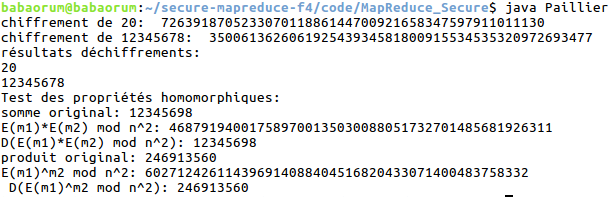
\includegraphics[scale=0.4]{img/res-paillier.png}
\caption{cryptosytème de Paillier et ses propriétés homomorphiques}
\label{Paillier}
\end{figure}



% ----------------------------------------------------------------------
	\subsection{Délivrables}
% ----------------------------------------------------------------------

Au cours de notre projet, de nombreuses réalisations nous ont été demandées pour que nos tuteurs puissent facilement utiliser MapReduce et comparer les résultats de leurs recherches. 
En plus de la mise en place du cluster, nous avons dû créer un programme qui permet d'installer et configurer hadoop : \textit{hadoopFromScratch.sh} (cf. \ref{hfs1}).
Il a fallu également réaliser des scripts qui permettent de lancer les jobs MapReduce en local et sur le cluster: \textit{launcher.sh} (cf. \ref{launcher1}), \textit{clusterLauncher.sh} (cf. \ref{clusterlauncher}).

 


% ----------------------------------------------------------------------
% Diagramme de Gantt réel
% ----------------------------------------------------------------------
\part{Diagrammes de Gantt}
%\includegraphics[
%    page=1,
%    width=\textwidth,
%    height=\textheight
%]{img/gantt-previ_cropped.pdf}
\includepdf[pages=-,scale=0.7, angle=90,pagecommand={\section{Diagramme prévisionnel}},height=\textheight, width=\textwidth]{img/gantt-previ_cropped.pdf}
\clearpage

%\includegraphics[
%    page=1,
%    height=\textheight,
%    width=\textwidth,
%    angle=90
%]{img/gantt-previ_cropped.pdf}
\includepdf[pages=-,scale=0.7, angle=90,pagecommand={\section{Diagramme réel}},height=\textheight, width=\textwidth]{img/gantt-cropped.pdf}

%%% CONCLUSION %%%%%%%%%%%%%%%%%%%%%%%%%%%%%%%%%%%%%%%%%%%%%%%%%%%%%%%%%
\bookmarksetup{startatroot}
\addtocontents{toc}{\bigskip}
\newpage
%\setcounter{section}{0}
\section{Conclusion}
%%%%%%%%%%%%%%%%%%%%%%%%%%%%%%%%%%%%%%%%%%%%%%%%%%%%%%%%%%%%%%%%%%%%%%%%
% CONCLUSION
%%%%%%%%%%%%%%%%%%%%%%%%%%%%%%%%%%%%%%%%%%%%%%%%%%%%%%%%%%%%%%%%%%%%%%%%
% TODO

Ceci clôture ce rapport de projet qui traite de la comparaison de complexité de deux méthodes utilisées pour la multiplication de matrices via MapReduce. Cette étude a été menée principalement sur un réseau de machines virtuelles, appelé \textit{cluster}, équipé du système d'exploitation Ubuntu et du framework Hadoop pré-installé. Au fil de ce rapport, nous avons présenté la théorie menée par nos tuteurs. Puis nous avons expliqué comment le \textit{namenode} a été configuré lors de sa création. Ceci afin de préparer les tâches MapReduce qui nous avait été demandé de programmer.\par
Notre objectif initial était de programmer en langage Java deux méthodes différentes de multiplication de matrices, celle demandant une seule étape map et reduce (\textit{One Step}) et celle en demandant deux (\textit{Two Steps}). Compte tenu de nos connaissances initiales dans les compétences qui étaient requises pour ce projet (Hadoop, Java, shell, Git, manipulation d'un cluster), cette première tâche a été réalisé en partie, non sans peine. Parmi les obstacles et principaux contretemps, les plus difficiles à résoudre ont concerné les problèmes internes au cluster. Plus de deux mois ont été nécessaires pour rechercher et assembler de nombreuses documentations sur l'ensemble du sujet. Pendant un autre mois, nous ne comprenions pas comment le HDFS fonctionnait, c'est pourquoi nous nous sommes résolus à faire les mesures sur nos ordinateurs personnelles en attendant le fonctionnement du cluster et du système distribué d'Hadoop.\par
D'après nos séries de mesure, bien que limité en ressources disponibles, nous avons su montrer que la courbe de complexité temporelle du job One Step sécurisé était asymptotiquement prépondérante devant celle du job non sécurisé. La pratique a confirmé le niveau de sécurité démontré par la théorie, de sorte qu'à partir d'aucune des valeurs d'une matrice placée en entrée il ne soit possible de connaître la valeur de l'autre matrice ou de celle en sortie. Le choix de grands nombres premiers permet le calcul de matrices comportant des valeurs élevés comme nous l'avons vu en Partie I.\par
Nous avons rapidement constaté une limite durant les tests, alors que nos tuteurs avaient prévus de rentrer des matrices assimilables aux données d'un système \textit{Big Data}, alors que le cluster est limité en disque dur, la taille maximale de matrices pouvant être traitées par le cluster se situe entre 450 et 500 lignes de valeurs. Nous pouvons comparer l'envergure de nos tests avec ceux de \textit{Google Labs}, le rapport des tests de multiplication de matrices publié sur internet rend compte de leur travail sur un cluster comportant 1800 machines constituées de processeurs Xeon (10 à 18 cœurs). Le cloud OpenStack du LIMOS ne nous délivrant pas des ressources comparables et par manque de temps, le nombre de mesures et le temps d'exécution des tâches MapReduce sont donc affectés.\par
Notre avancement dans le projet nous a permis de programmer et optimiser l'algorithme du One Step, cependant de nombreuses autres perspectives sont envisageables:
\begin{itemize}
\item Finir l'algorithme Java de la multiplication de matrices en deux étapes (Two Steps) que nous avons commencé.
\item Effectuer le même travail de mesures sur cette méthode et la méthode sécurisée associée.
\item Comparer les complexités temporelles du One Step et du Two Steps.
\item Implémenter l'approche Collision-Resistant-Secure-Private (CRSP).
\item Rechercher les courbes théoriques se rapprochant le plus des courbes expérimentales.
\end{itemize}

%%% BIBLIOGRAPHY %%%%%%%%%%%%%%%%%%%%%%%%%%%%%%%%%%%%%%%%%%%%%%%%%%%%%%%
\newpage
\thispagestyle{plain}
\pagenumbering{alph}

\section*{Références bibliographiques}

\addcontentsline{toc}{section}{Références bibliographiques}
\nocite{*}
\printbibliography


%%% ANNEXES %%%%%%%%%%%%%%%%%%%%%%%%%%%%%%%%%%%%%%%%%%%%%%%%%%%%%%%%%%%%
\appendix
\newpage
\pagenumbering{Roman}
\part{Annexe}

\section{Documentation des scripts et programmes réalisés}

	\subsection{Script automatisant un job MapReduce sur le cluster: clusterLauncher.sh}
    \label{clusterlauncher}
  	\begin{center}
        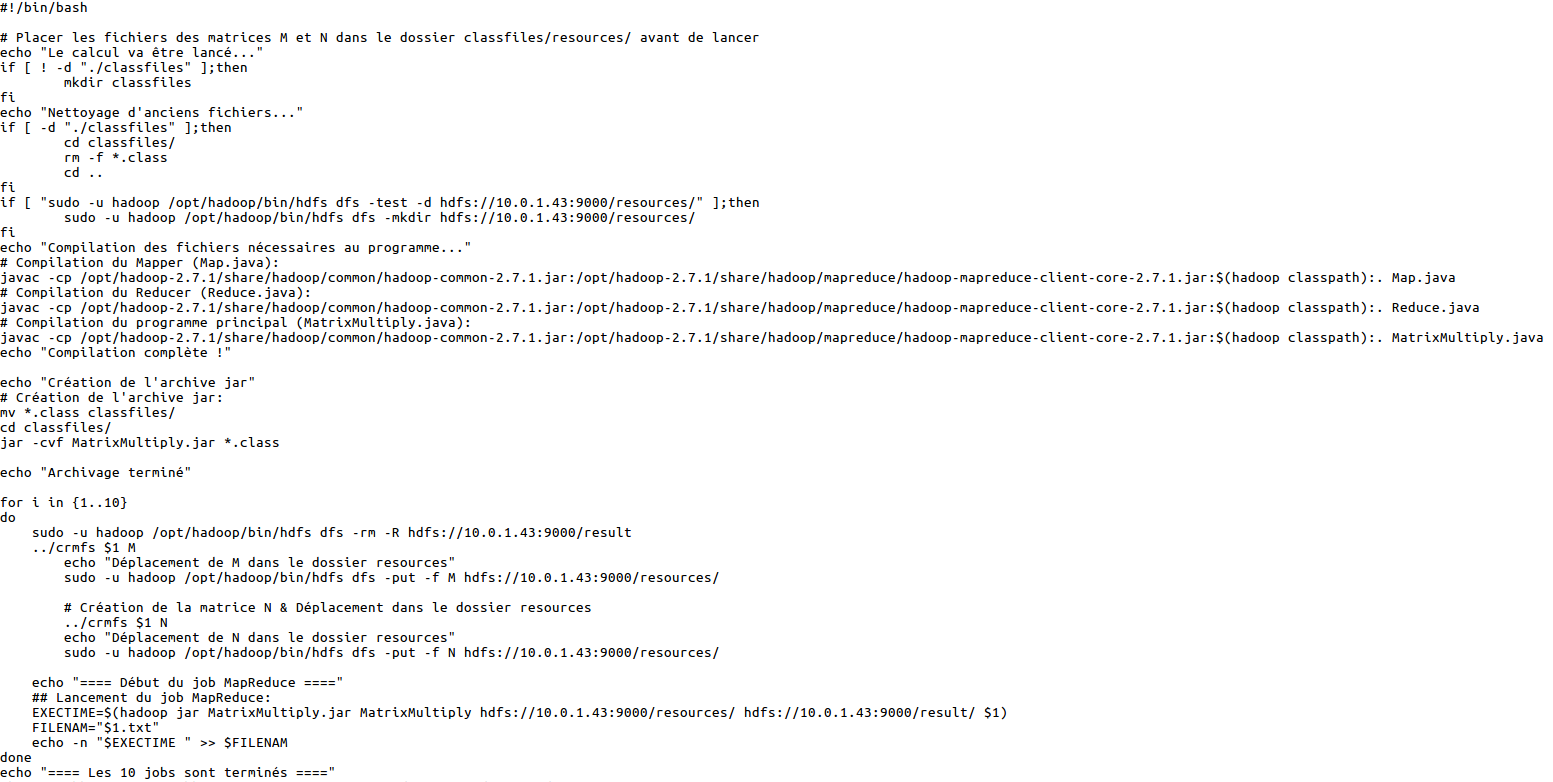
\includegraphics[scale=0.38, angle=90]{./img/codeClusterLauncherOSNS.png}
        \begin{turn}{90}
        \begin{minipage}{\linewidth}
        \vspace{2\baselineskip}
        Ce bash permet le lancement d'une multiplication de matrices avec MapReduce en une seule étape sur le cluster. Il prend en paramètre le nombre de lignes/colonnes que doivent posséder les matrices à générer.
		\end{minipage}
        \end{turn}
    \end{center}
    
	\subsection{Installation automatique d'hadoop dans une VM vierge: hadoopFromScratch.sh}
    \vspace{2\baselineskip}
    \label{hfs1}
  	\begin{center}
        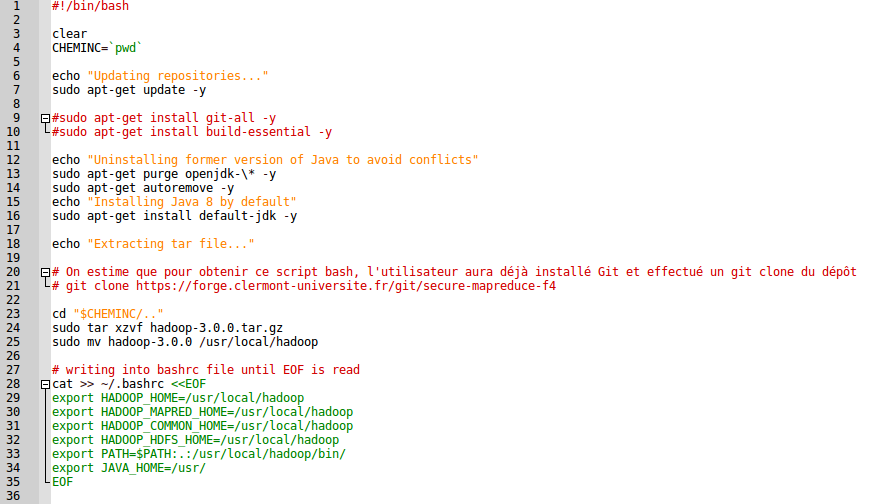
\includegraphics[scale=0.7, angle=90]{./img/hfs1.png}
    \end{center}
    \vspace{2\baselineskip}
    \clearpage

    \label{hfs2}
  	\begin{center}
        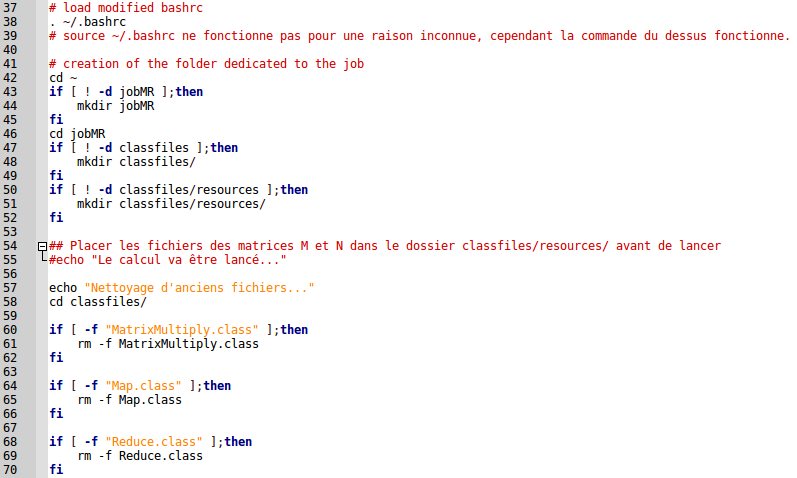
\includegraphics[scale=0.75, angle=90]{./img/hfs2.png}
    \end{center}
    \vspace{2\baselineskip}

    \label{hfs3}
  	\begin{center}
        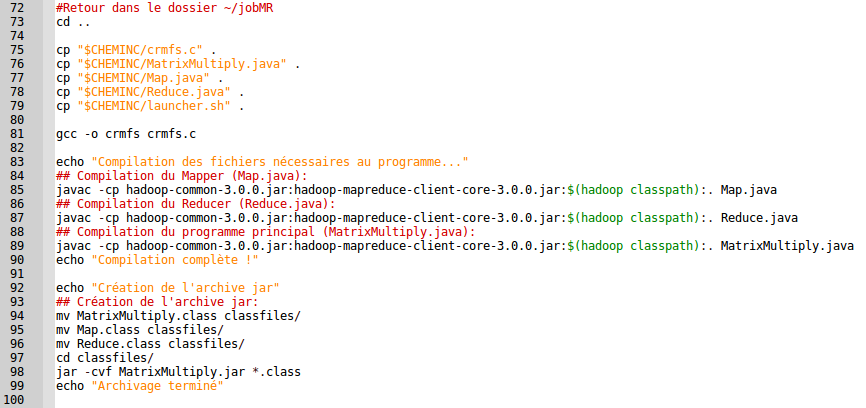
\includegraphics[scale=0.75, angle=90]{./img/hfs3.png}
    \end{center}   
    
    \label{hfs4}
  	\begin{center}
        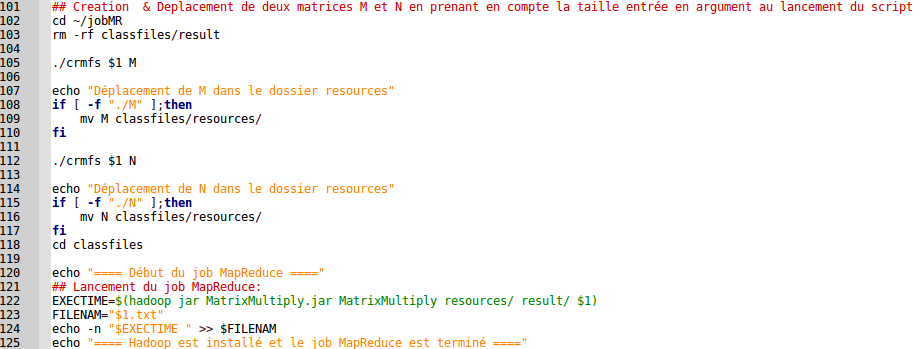
\includegraphics[scale=0.7, angle=90]{./img/hfs4.png}
    \end{center}
    \vspace{2\baselineskip}
    \clearpage    
    
    \subsection{Script permettant le lancement d'un job MapReduce en local: launcher.sh}    
    \label{launcher1}
    \begin{flushleft}
    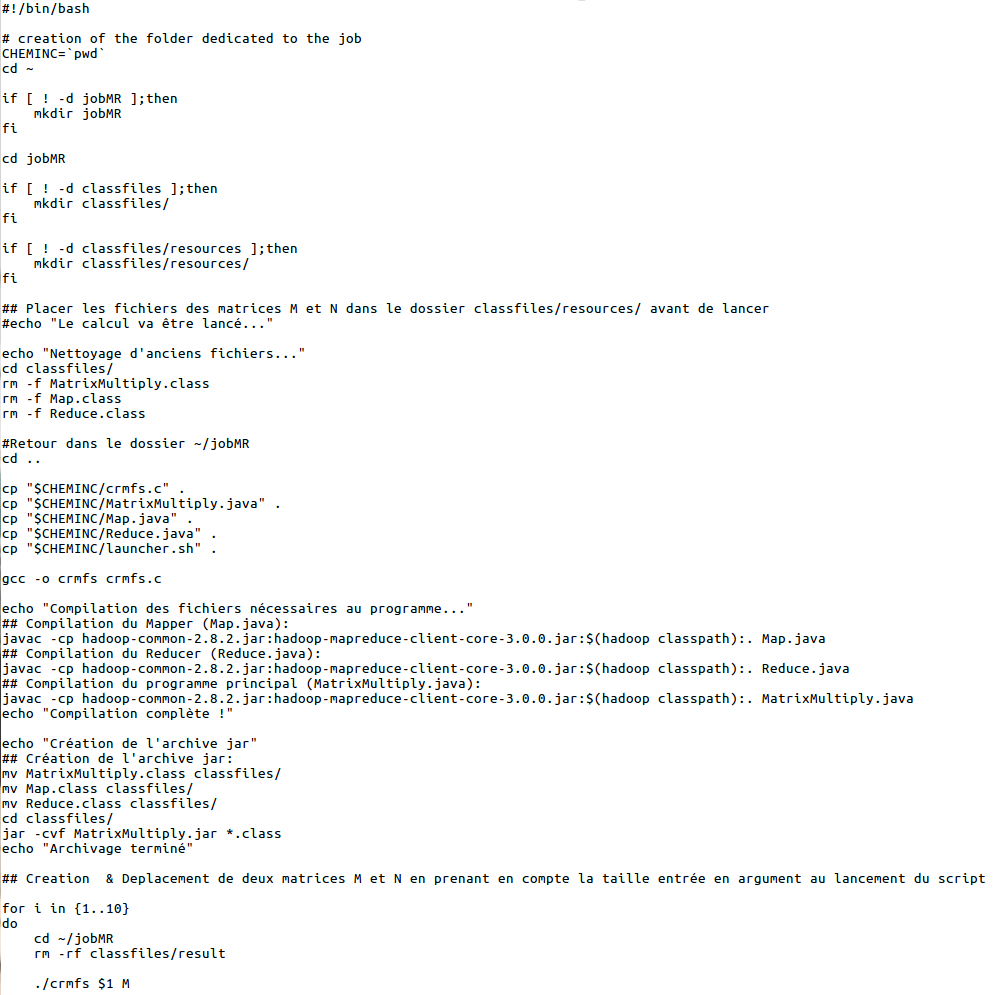
\includegraphics[scale=0.45, angle=0]{./img/codeLauncherP1.png}
    \end{flushleft}
    
    \label{launcher2}
        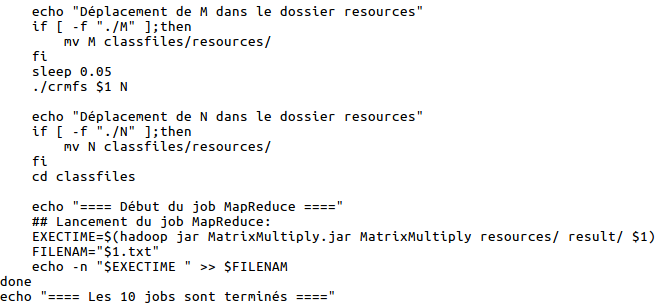
\includegraphics[scale=0.65, angle=0]{./img/codeLauncherP2.png}
        \vspace{1\baselineskip}
        
Ce script nécessite un PC possédant le système d'exploitation Linux et Hadoop. Si cela n'est pas déjà fait, il est possible de tout installer et configurer grâce au script \textit{hadoopFromScratch.sh}. Ce bash permet le lancement d'une multiplication de matrices avec MapReduce en une seule étape. Il prend en paramètre le nombre de lignes/colonnes que doivent posséder les matrices à générer.

Jusqu'à la compilation des fichiers Java, il s'agit des mêmes lignes de code que le fichier \textit{hadoopFromScratch} (cf. \ref{hfs1})
\clearpage
    
    \subsection{Automatisation des calculs statistiques: Stat.sh}
    \vspace{2\baselineskip}
    \label{Stat.sh}
  	\begin{center}
        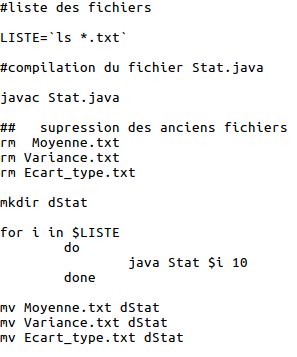
\includegraphics[scale=0.8, angle=0]{./img/scriptStat.png}
    \end{center}
\clearpage

	\subsection{Générer des matrices aléatoires: crmfs.c}
    \vspace{2\baselineskip}
    \label{crmfs.c}
  	\begin{center}
        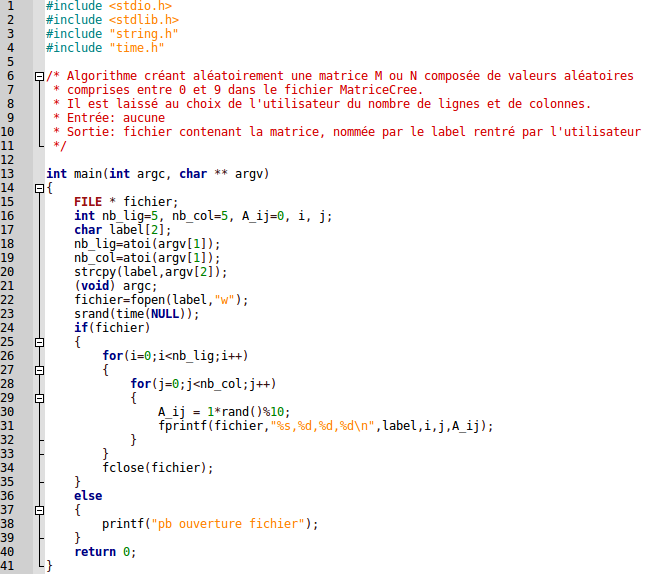
\includegraphics[scale=0.6, angle=0]{./img/crmfs.png}
    \end{center}
    \vspace{2\baselineskip}
    Ce code permet de générer une matrice dans un fichier sans extension sous la forme de plusieurs vecteurs. Une fois compilé, le fichier exécutable nécessite deux arguments: le nombre de lignes/colonnes d'une matrice et son nom. Le nom de la matrice permet de remplir la première chaîne de caractères de chaque vecteur et de nommer le fichier résultant de la fonction. Chaque matrice générée est carrée et comprend des nombres aléatoires d'entiers compris entre 0 et 9.
\clearpage

%	\subsection{Mapper du job Mapreduce One Step non sécurisé: Map.java}
%    \vspace{2\baselineskip}
%    \label{mapns}
%  	\begin{center}
%        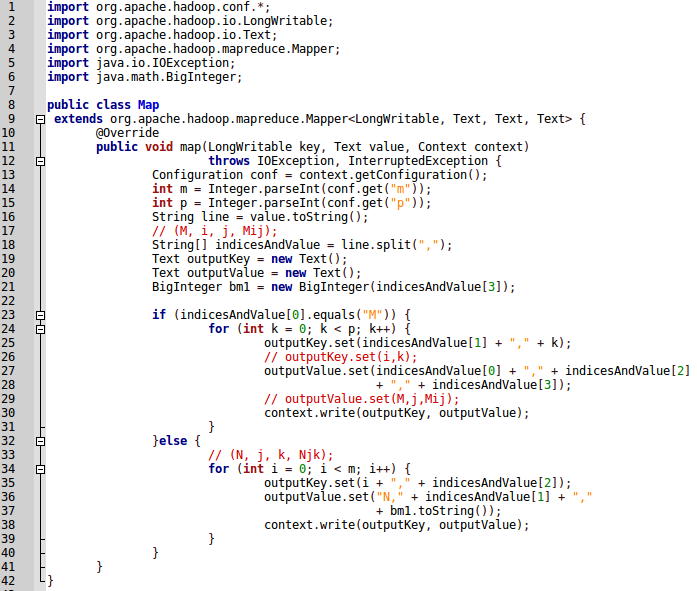
\includegraphics[scale=0.65, angle=0]{./img/MapNS.png}
%    \end{center}
%    \vspace{2\baselineskip}
%\clearpage	
	
%	\subsection{Mapper du job Mapreduce One Step sécurisé: Map.java}
%    \vspace{2\baselineskip}
%    \label{secumap}
%  	\begin{center}
%        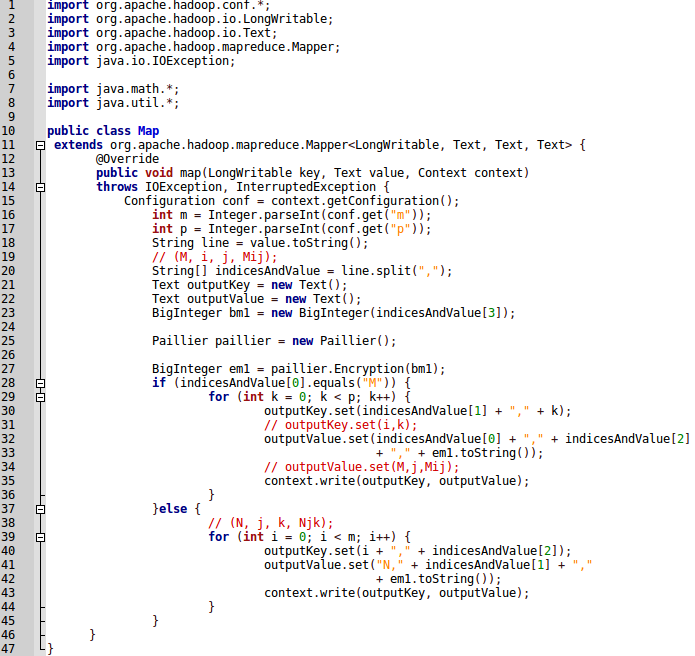
\includegraphics[scale=0.65, angle=0]{./img/MapSecu.png}
%    \end{center}
%    \vspace{2\baselineskip}
%\clearpage
%	
%	\subsection{Driver commun aux jobs sécurisés et non sécurisés: MatrixMultiply.java}
%    \vspace{2\baselineskip}
%    \label{Matmult}
%  	\begin{center}
%        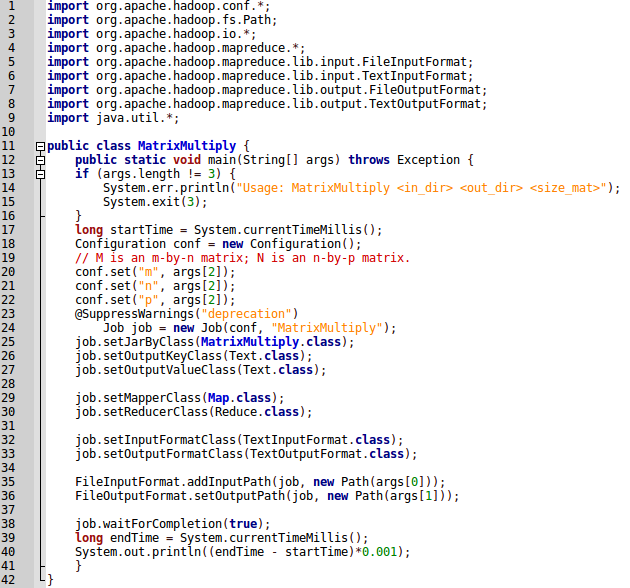
\includegraphics[scale=0.7, angle=0]{./img/MatrixMultiplyCommun.png}
%    \end{center}
%	
%	\subsection{Chiffrement de valeurs par le cryptosystème: Paillier.java}
%    \vspace{2\baselineskip}
%    \label{paillier1}
%  	\begin{center}
%        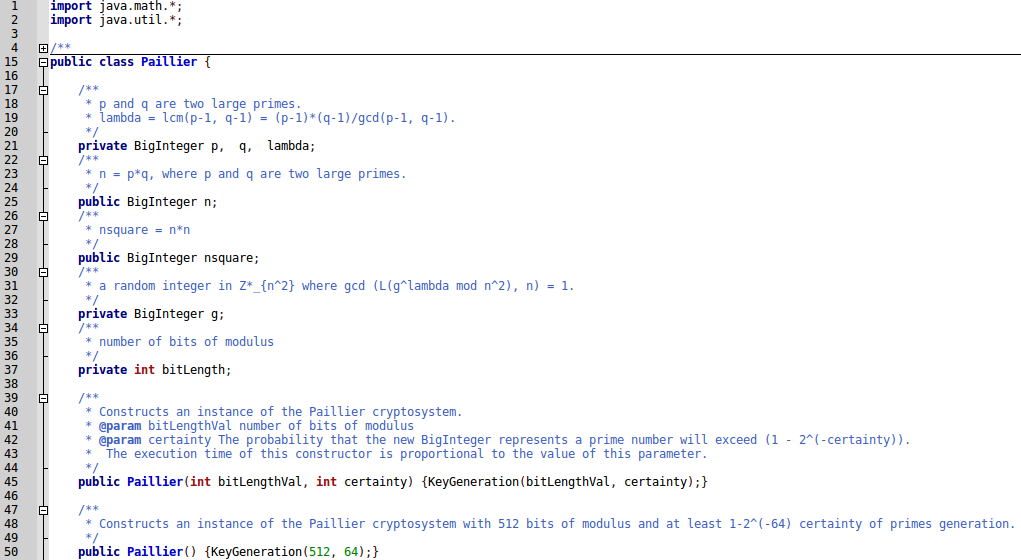
\includegraphics[scale=0.6, angle=90]{./img/Paillier1.png}
%    \end{center}
%    \vspace{2\baselineskip}
%    \clearpage
%    
%    \vspace{2\baselineskip}
%    \label{paillier2}
%  	\begin{center}
%        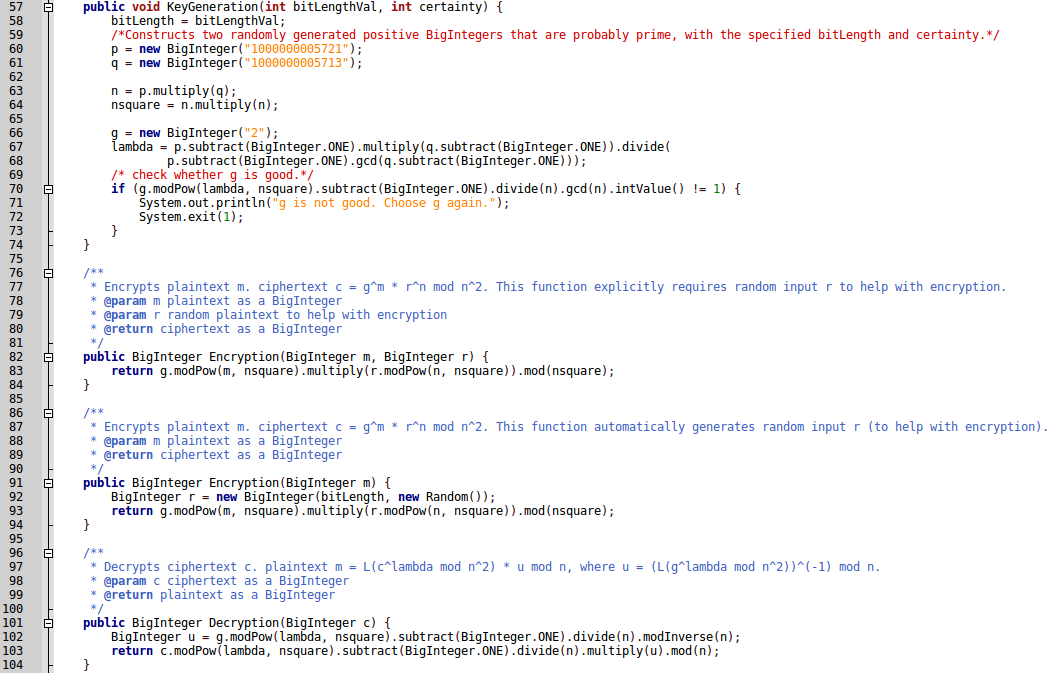
\includegraphics[scale=0.6, angle=90]{./img/Paillier2.png}
%    \end{center}
%    \vspace{2\baselineskip}
%    \clearpage
%    
%    \vspace{2\baselineskip}
%    \label{paillier3}
%  	\begin{center}
%        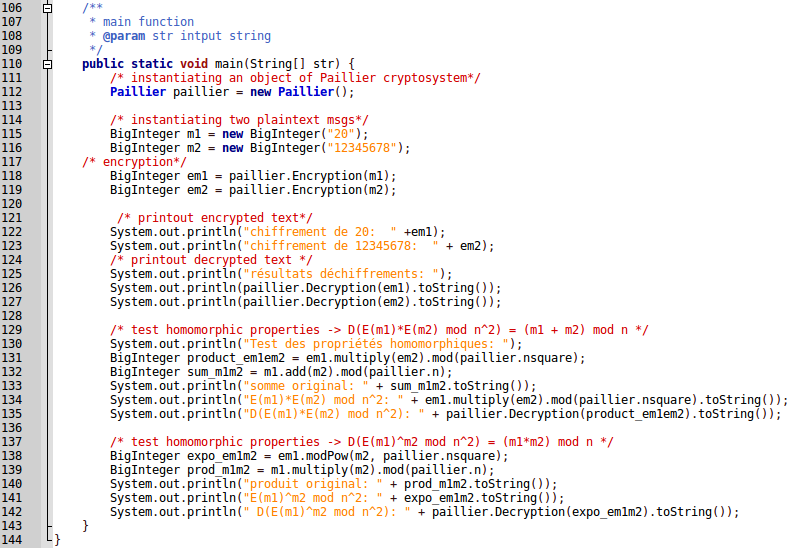
\includegraphics[scale=0.8, angle=90]{./img/Paillier3.png}
%    \end{center}
%    \vspace{2\baselineskip}
%    \clearpage
%    
%	\subsection{Reducer du job Mapreduce One Step non sécurisé: Reduce.java}
%    \vspace{2\baselineskip}
%    \label{reduceNS}
%  	\begin{flushleft}
%        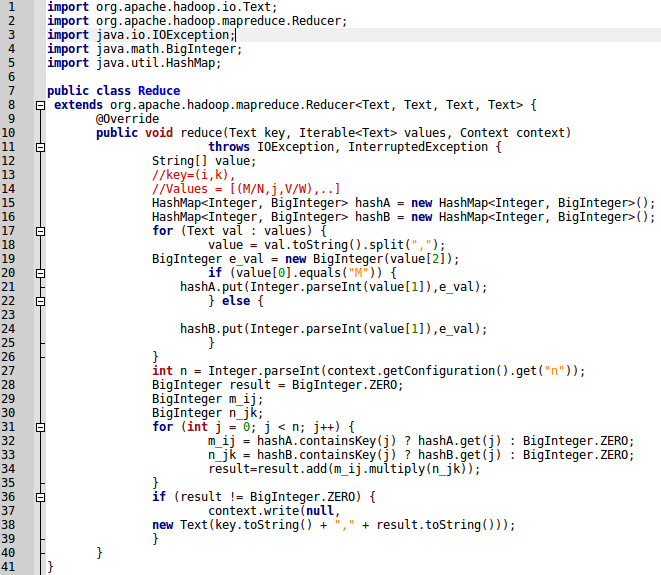
\includegraphics[scale=0.7, angle=0]{./img/ReduceNS.png}
%    \end{flushleft}
%    
%    \subsection{Reducer du job Mapreduce One Step sécurisé: Reduce.java}
%    \vspace{2\baselineskip}
%    \label{reduceSecu}
%  	\begin{center}
%        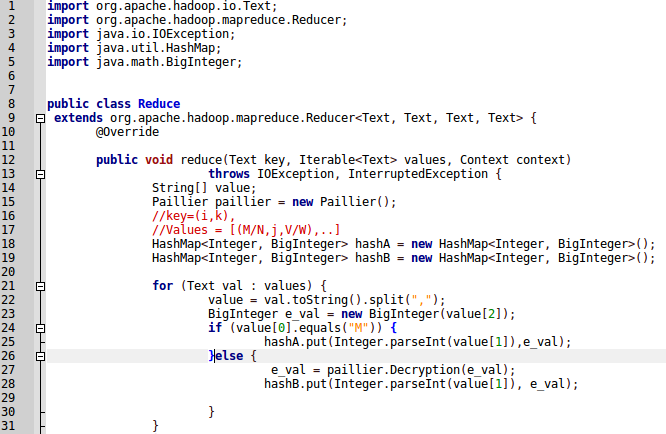
\includegraphics[scale=0.9, angle=90]{./img/ReduceSecu.png}
%    \end{center}
%
%    \label{reduceSecu}
%  	\begin{center}
%        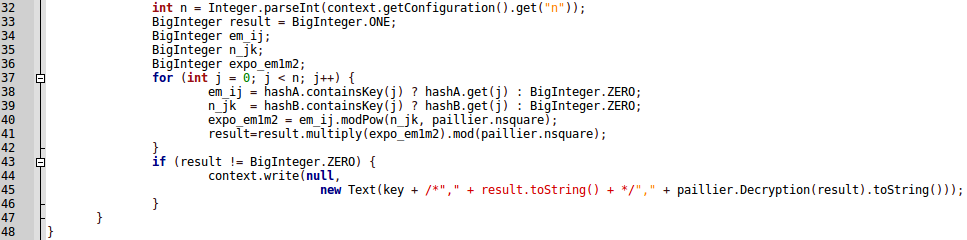
\includegraphics[scale=0.7, angle=90]{./img/ReduceSecu2.png}
%    \end{center}
%    \vspace{2\baselineskip}
%    \clearpage
    
    \subsection{Calcul des moyennes, écarts-types et variances: Stat.java}
    \vspace{2\baselineskip}
    \label{stat1}
  	\begin{center}
        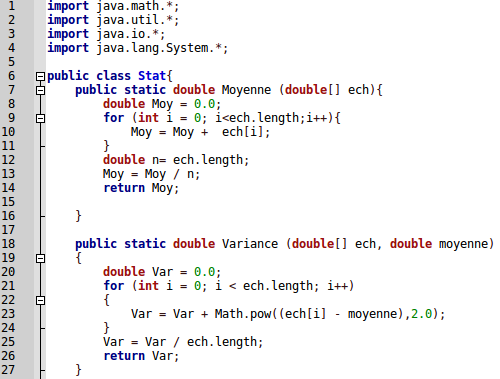
\includegraphics[scale=0.9, angle=90]{./img/Stat1.png}
    \end{center}
    \vspace{2\baselineskip}
    \clearpage
    
    \vspace{2\baselineskip}
    \label{stat2}
  	\begin{center}
        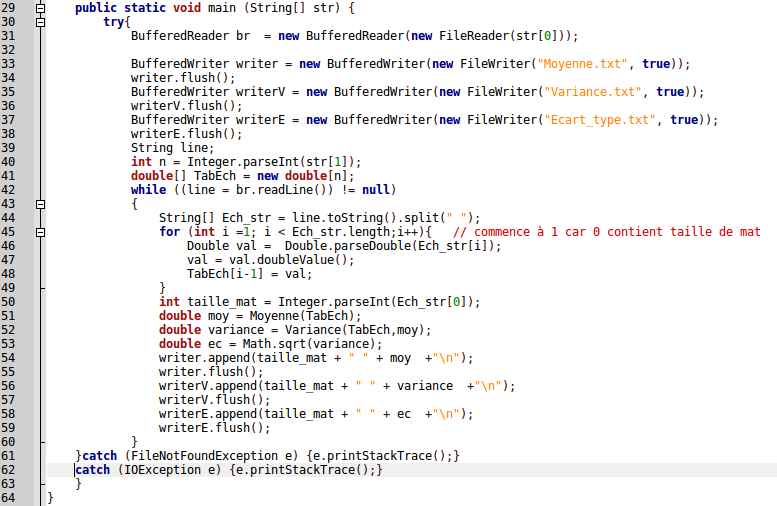
\includegraphics[scale=0.8, angle=90]{./img/Stat2.png}
    \end{center}
    \vspace{2\baselineskip}
    \clearpage
    
\section{Mesures}
	\subsection{séries de mesures}
	\label{txtmesures10jobs}
	\begin{center}
		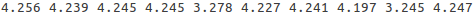
\includegraphics[scale=0.9, angle=0]{./img/fichier57.png}
		Temps d'exécutions en secondes des 10 jobs lancés pour des matrices constituées de 57 lignes et colonnes.
	\end{center}
	
	\subsection{moyenne des mesures pour chaque taille de matrice}
	\label{txtmesuresMoy}
	\begin{center}
		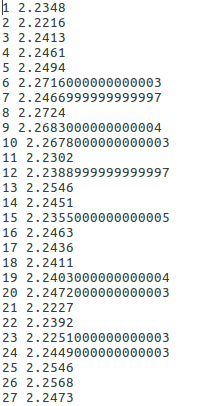
\includegraphics[angle=0]{./img/extraitMoyTri.png}\par
		Extrait du fichier stockant la taille des matrices en première colonne et la moyenne des 10 valeurs lues dans chaque fichier de mesures.
	\end{center}
	\clearpage
	
	\subsection{variance des mesures pour chaque taille de matrice}
	\label{txtmesuresVar}
	\begin{center}
		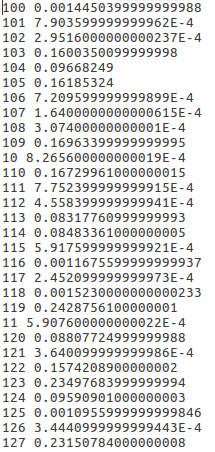
\includegraphics[angle=0]{./img/extraitVariance.png}\par
		Extrait du fichier composé des variances des échantillons de mesure calculés sur la multiplication de matrices en une étape.
	\end{center}
	
	\label{txtmesures}
	\begin{center}
	\subsection{Courbe des benchmarks sur le job One Step}	
	\vspace{2\baselineskip}
	\includegraphics[
    page=1,
    width=15cm,
    height=15cm,
]{courbesOneStep.pdf}		
	\end{center}
\end{document}
